\documentclass[UTF8,a4paper,15pt,titlepage,oneside]{ctexbook}
\usepackage{listings}
\usepackage{xcolor}
\usepackage{booktabs}
\usepackage{float}
\usepackage{amsmath}
\usepackage{amssymb}
\usepackage{geometry}
\usepackage{graphicx}
\usepackage{hyperref}
\usepackage{enumerate}
\usepackage{fancyhdr}
\usepackage{setspace}
\usepackage{cite}
\usepackage{listings}
\usepackage{appendix}
\usepackage{titlesec}
\usepackage{indentfirst}
\usepackage{fixltx2e}
\usepackage{mdframed}
\usepackage{subcaption}
\usepackage[table]{xcolor}
\usepackage{booktabs}

\fancyfoot[LE,RO]{\thepage}
\setcounter{secnumdepth}{3}
\geometry{left=2cm, right=2cm, top=3cm, bottom=3cm}
\newcommand{\superscript}[1]{\textsuperscript{#1}}
\renewcommand\thesection{\arabic {section}}

\setstretch{1.5}
\lstset{ 
  basicstyle=\ttfamily\small,   % 基本字体样式
  numbers=left,                 % 行号在左侧显示
  numberstyle=\tiny\color{gray},% 行号字体样式
  stepnumber=1,                 % 行号的步长
  numbersep=5pt,                % 行号与代码间的距离
  backgroundcolor=\color{lightgray}, % 背景颜色
  showspaces=false,             % 不显示空格
  showstringspaces=false,       % 不显示字符串中的空格
  showtabs=false,               % 不显示制表符
  frame=single,                 % 单线框
  rulecolor=\color{black},      % 框的颜色
  tabsize=2,                    % 制表符大小
  captionpos=b,                 % 标题位置
  breaklines=true,              % 自动换行
  breakatwhitespace=false,      % 仅在空格处换行
  title=\lstname                % 文件名作为标题
}


\pagestyle{fancy}
\fancyhf{}
\fancyhead[L]{\text{《AI导论》}}
\fancyhead[R]{\text{智能舆情分析系统及其在汽车品牌管理中的应用}}
\fancyfoot[C]{\thepage}


\bibliographystyle{gbt7714-numerical}


\hypersetup{hidelinks}


\titleformat{\section}
  {\centering\zihao{3}\heiti} 
  {第\chinese{section}章}
  {1em} 
  {} 

\titlespacing*{\section}
  {0pt} 
  {2em} 
  {2em}

\titleformat{\subsection}
  {\raggedright\zihao{4}\heiti} 
  {\arabic{section}.\arabic{subsection}}
  {1em}
  {}

\titlespacing*{\subsection}
  {0pt}
  {1.5em}
  {0.75em}

\titleformat{\subsubsection}
  {\raggedright\zihao{-4}\heiti}
  {\arabic{section}.\arabic{subsection}.\arabic{subsubsection}}
  {1em}
  {}

\titlespacing*{\subsubsection}
  {0pt}
  {1.2em}
  {0.6em}

\begin{document}


\begin{titlepage}

        

        
        \begin{figure}[h]
          \begin{flushleft}
              
\includegraphics[width=0.2\textwidth, keepaspectratio=false]{pictures/44.png} % 修改为实际图片路径
          \end{flushleft}
      \end{figure}
        
        \begin{center}

        \begin{figure}[H]
          \centering
          
\includegraphics[width=0.7\textwidth,keepaspectratio=false]{pictures/43.png} % 修改为实际图片路径
      
        \end{figure}
        \vspace*{2cm}
        {\Huge \textbf{智能舆情分析系统}}
        \vspace{0.3cm}

        {\Huge \textbf{及其在汽车品牌管理中的应用}}
        
        \vspace{1cm}
        
        {\Large 王肖鉴\;徐思睿\;方俊皓\;冯越\;梁启宸}

        
        \vfill

        {\Large 2024年6月10日}
        
        
        
        \vspace{1cm}
        
        
        
        
        
        
        \vfill
      \end{center}
\end{titlepage}
\newpage
\begin{titlepage}
  \vspace*{2cm}
  \begin{center}
    \textbf{\zihao{4}摘要}

        

        \vspace{0.1cm}
        \end{center}

        随着互联网和社交媒体的迅猛发展,大量的舆论数据不断涌现,形成了海量且复杂的数据信息流。这些数据不仅包含了丰富的内容,更是反映了社会各阶层、各领域的意见和情感,对于深入理解公众情绪和引导社会舆论具有重要的战略意义。
        
        本研究旨在设计并实现一个智能舆情分析系统,通过集成最新的技术和算法,全面提升舆情数据的采集、处理、分析和展示能力。
        
        系统架构包括数据采集层、数据处理层、分析层和展示层。数据采集层利用爬虫技术从各种数据源获取原始数据,数据处理层对采集到的原始数据进行预处理,包括数据清洗、去重和分词处理等。
        分析层通过多种分析模型对处理后的数据进行深入分析,包括关键词提取、主题分析和情感分析。展示层通过可视化工具将分析结果以直观的形式展示给用户,帮助用户更好地理解和利用舆情数据。
        
        本研究还进行了实例应用,展示了智能舆情分析系统在汽车品牌管理中的有效性和实用性。
        
        \vspace{1cm}
        \noindent
        \textbf{\zihao{5}关键词}\;\;舆情分析,情感分析,热点分析,主题分析,深度学习

\end{titlepage}
\newpage
\begin{titlepage}
  \vspace*{2cm}
  \begin{center}
    \textbf{\zihao{4}Abstract}

        

        \vspace{0.1cm}
        \end{center}

        With the rapid development of the Internet and social media, a large amount of public opinion data is continuously emerging, forming a massive and complex information flow. This data not only contains rich content but also reflects the opinions and emotions of various social strata and fields, which is of great strategic significance for deeply understanding public sentiment and guiding social opinion. 
        
        This study aims to design and implement an intelligent public opinion analysis system by integrating the latest technologies and algorithms to comprehensively enhance the capabilities of opinion data collection, processing, analysis, and presentation. 
        
        The system architecture includes a data collection layer, a data processing layer, an analysis layer, and a presentation layer. The data collection layer uses crawler technology to obtain raw data from various data sources. The data processing layer preprocesses the collected raw data, including data cleaning, deduplication, and word segmentation. The analysis layer conducts in-depth analysis of the processed data through various analytical models, including keyword extraction, topic analysis, and sentiment analysis. The presentation layer uses visualization tools to present the analysis results to users in an intuitive form, helping them better understand and utilize public opinion data. 
        
        This study also conducted a case application, demonstrating the effectiveness and practicality of the intelligent public opinion analysis system in car brand management.

\vspace{1cm}
\noindent
\textbf{\zihao{5}keywords:}\;\;public opinion analysis, sentiment analysis, hot topic analysis, topic modeling, deep learning



\end{titlepage}
\clearpage
\tableofcontents
\clearpage
\section{引言}

\subsection{研究背景}

随着互联网和社交媒体的迅猛发展,大量的舆论数据不断涌现,形成了海量且复杂的数据信息流。这些数据不仅包含了丰富的内容,更是反映了社会各阶层、各领域的意见和情感,对于深入理解公众情绪和引导社会舆论具有重要的战略意义。

首先,舆论数据涵盖了从宏观的社会议题到微观的个体观点的广泛信息,能够全面展示社会各个层面的关注焦点和情感倾向。通过对这些数据的深入挖掘和分析,能够洞察到不同人群、不同地域和不同行业的需求和情感变化,从而为决策者提供有力的支持。

其次,舆论数据的实时性和动态性,使其成为社会事件和公共政策的风向标。通过实时监测和分析舆论数据,能够及时捕捉到社会情绪的变化趋势,预见潜在的舆情风险,并制定相应的应对策略。这对于公共管理、危机应对和品牌管理等领域,都是至关重要的。

此外,舆论数据的多样性和复杂性,要求我们采用先进的数据处理和分析技术,如大数据分析、自然语言处理和深度学习等,以提升对数据的洞察力和决策的科学性。通过建立完善的舆情分析体系,不仅能够提高信息处理的效率,还能够深度挖掘数据背后的潜在规律,提供更为精准的舆情预测和洞察。

\begin{figure}[H]
  \centering
  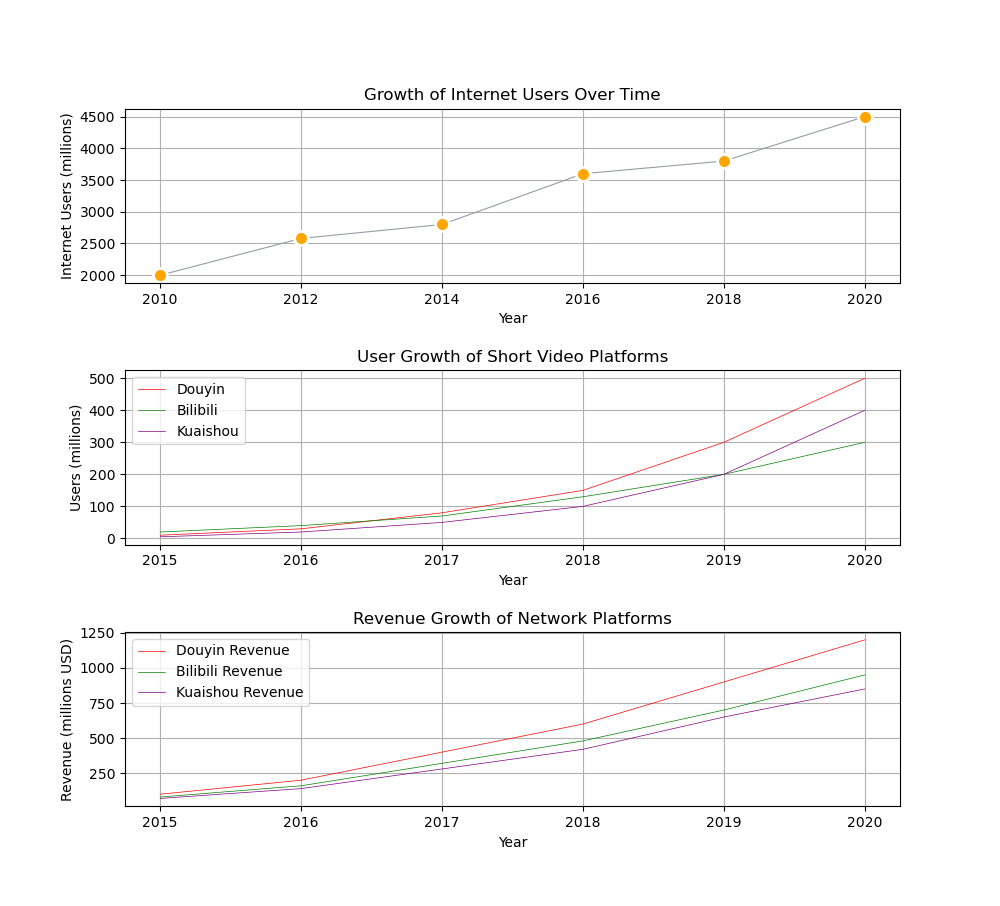
\includegraphics[width=0.7\textwidth,keepaspectratio=false]{pictures/10.png} % 修改为实际图片路径
  \caption{互联网和社交媒体的快速发展}
  
\end{figure}

然而,传统的舆情分析方法因处理能力有限,
难以有效应对海量数据和复杂的信息结构,故对智能化、
自动化的舆情分析系统的需求日益增长。

\subsection{研究现状与先行研究综述}

在现有的研究中,虽然已经有许多工具和模型被提出来用于处理特定的舆情分析任务,
如情感分析、话题检测等,
但这些方法往往孤立地看待问题,缺乏一个统一的、
综合的分析框架来处理从数据采集到舆情预测的全流程。
此外,大多数系统未能有效利用最新的深度学习技术和大规模预训练模型,
从而限制了分析的深度和准确性。

\subsection{研究目的}

本研究旨在设计并实现一个智能舆情分析系统,通过集成最新的技术和算法,
全面提升舆情数据的采集、处理、分析和展示能力。
研究的目的在于通过构建一个高效的数据采集层,
利用先进的分词和特征提取技术优化数据处理过程,
并通过深度学习模型和大模型提高情感分析和趋势预测的精度与深度。

\subsection{研究意义}


本研究的意义在于为政府机关、企业和公众提供一个强有力的决策支持工具,
帮助他们更好地理解和应对公众舆论,预测和引导舆情的发展方向。
通过实时监控和全面分析舆情数据,该系统不仅能够增强社会舆论管理的科学性和有效性,
也为舆情研究领域提供了新的技术应用示范。

综上所述,本研究填补了现有舆情分析方法的不足,提出了一个全面且高效的解决方案,
对于提高舆情分析的实时性和准确性具有重要的研究和应用价值。

\section{系统架构概述}

本研究设计并实现了一种先进的智能舆情分析系统,旨在识别热点话题、分析情感倾向并追踪舆情变化趋势。系统架构包括数据采集层、数据处理层和分析层,通过集成爬虫技术、分词模型、特征提取模型、深度学习模型以及大模型来实现综合分析。


\begin{figure}[H]
  \centering
  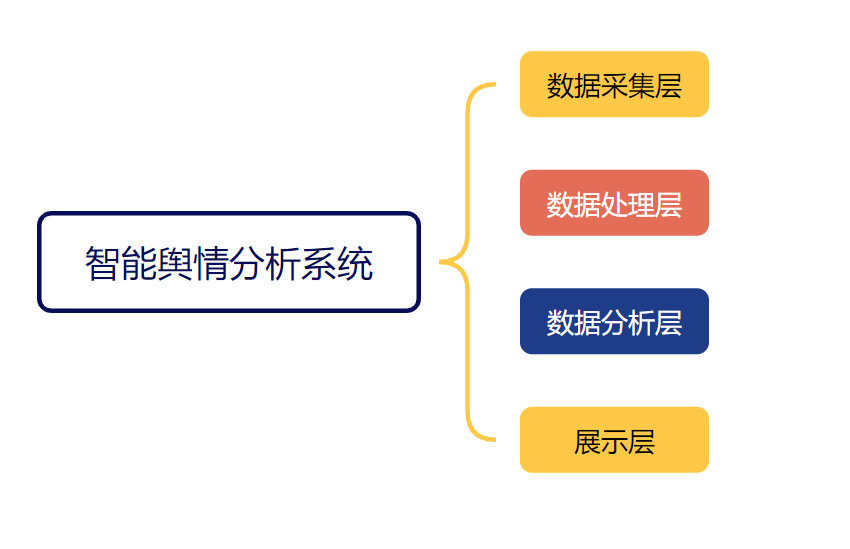
\includegraphics[width=0.7\textwidth,keepaspectratio=false]{pictures/45.png} % 修改为实际图片路径
  \caption{系统组成}
  
\end{figure}


\subsection{数据采集层}

数据采集层是系统的基础,负责从各种数据源中获取原始数据。这些数据源包括社交媒体平台(如微博)、新闻网站等。为了保证数据的全面性和实时性,系统使用了多种爬虫技术和API接口。


\vskip 0.2cm
\noindent
\textbf{数据来源:}

\begin{enumerate}[\textbullet]
  \item 社交媒体平台:如微博、微信、Twitter等。
  \item 新闻网站:如新华网、人民网、BBC等。
  \item 博客和评论网站:如豆瓣、知乎等。
\end{enumerate}

\vskip 0.2cm
\noindent
\textbf{数据收集:}

\begin{enumerate}[\textbullet]
  \item 使用Scrapy等爬虫框架,编写爬虫脚本,定期或实时抓取数据。
  \item 利用API接口,直接获取数据源提供的结构化数据。通过爬虫技术从多个平台实时收集数据,确保数据的丰富性和多样性。
  \item 数据更新:定期或实时更新数据,保持系统数据的最新状态。
  \item 协作影响:数据采集层为数据处理层提供基础数据,采集的原始数据必须全面、及时和准确,才能保证后续处理和分析的有效性。
\end{enumerate}

\subsection{数据处理层}

数据处理层对采集到的原始数据进行预处理,这是保证数据质量和分析准确性的关键步骤。预处理包括数据清洗、去重和分词处理等。

\vskip 0.2cm
\noindent
\textbf{数据清洗:}

\begin{enumerate}[\textbullet]
  \item 去除广告、垃圾信息以及无关信息,确保数据的纯净。标记和处理缺失值,填补或删除不完整的数据记录。
\end{enumerate}

\vskip 0.2cm
\noindent
\textbf{数据去重:}

\begin{enumerate}[\textbullet]
  \item 利用哈希算法去重,避免重复数据影响分析结果。
\end{enumerate}

\vskip 0.2cm
\noindent
\textbf{分词处理:}

\begin{enumerate}[\textbullet]
  \item 使用Jieba分词工具对文本进行分词,将文本拆分为有意义的词语。
\end{enumerate}

\vskip 0.2cm
\noindent
\textbf{层级交互:}

\begin{enumerate}[\textbullet]
  \item 数据处理层为数据分析层提供清洁和结构化的数据,处理质量直接影响分析结果的准确性。
  \item 数据处理层也反馈给数据采集层,帮助优化数据采集策略,确保获取到的数据更符合分析需求。

\end{enumerate}

\subsection{数据分析层}

数据分析层是系统的核心,通过多种分析模型对处理后的数据进行深入分析,包括关键词提取、主题分析和情感分析。

\vskip 0.2cm
\noindent
\textbf{关键词提取:}

\begin{enumerate}[\textbullet]
  \item 采用TF-IDF(Term Frequency-Inverse Document Frequency)方法,将文本转化为特征向量,识别出文本中的重要关键词。
\end{enumerate}

\vskip 0.2cm
\noindent
\textbf{主题分析:}

\begin{enumerate}[\textbullet]
  \item 采用BERT嵌入与TF-IDF特征提取方式结合,利用朴素贝叶斯分类器进行有监督学习的主题分类
  \item 利用LDA(Latent Dirichlet Allocation)模型对文本进行主题建模,提取出具有代表性的热点话题。
\end{enumerate}

\vskip 0.2cm
\noindent
\textbf{情感分析:}

\begin{enumerate}[\textbullet]
  \item 结合BERT嵌入(Bidirectional Encoder Representations from Transformers)对文本进行特征提取
  \item 采用深度学习模型(如RNN、CNN),对文本进行情感分类,区分正面、中性和负面情感
\end{enumerate}

\vskip 0.2cm
\noindent
\textbf{趋势分析:}

\begin{enumerate}[\textbullet]
  \item 使用时间序列模型(如ARIMA)对舆情数据进行趋势预测,分析舆情的发展方向。

\end{enumerate}

\subsection{展示层}

展示层通过可视化工具将分析结果以直观的形式展示给用户,帮助用户更好地理解和利用舆情数据。这一层次主要使用D3.js和Echarts等可视化工具。

\vskip 0.2cm
\noindent
\textbf{可视化报告:}

\begin{enumerate}[\textbullet]
  \item 生成交互式图表和报告,直观展示数据分析结果。
\end{enumerate}

\vskip 0.2cm
\noindent
\textbf{综合分析:}

\begin{enumerate}[\textbullet]
  \item 整合热点话题、情感分析和趋势预测的结果,提供全面的舆情洞察,帮助决策者做出更明智的决策。
\end{enumerate}


\section{数据采集层}

我们本次研究的数据主要来源于网络爬虫,以下为选择爬虫技术的主要依据:

爬虫技术能够从广泛的互联网资源中获取数据,这些数据来源覆盖面广,帮助我们了解不同群体的观点和情感倾向。通过爬虫技术,我们可以确保分析的全面性和深入性。


此外,互联网数据更新频率极高,信息动态变化迅速。爬虫技术能够定期或实时地抓取最新数据,这对于舆情监控、市场趋势分析等需要实时数据的应用场景尤为重要。通过不断获取最新数据,我们的模型可以及时反映当前的趋势和变化,保持高效的适应性和响应速度。
通过爬虫技术,我们可以自动化地、大规模地收集数据,能够为机器学习模型提供充足的训练样本,从而提升模型的准确性和泛化能力。

不仅如此,爬虫技术能够从不同的网站和平台获取数据,这意味着我们可以获得多样化的数据样本。这种多样性有助于提高数据的代表性,使得训练模型能够适用于更广泛的应用场景。例如,在情感分析中,不同平台上的用户评论可能具有不同的表达方式和情感倾向,通过多样化的数据,我们可以训练出更具鲁棒性和通用性的模型。

\subsection{数据来源}

数据采集的目标是从互联网获取高质量的大数据,以支持后续的分析和模型训练。常用的数据来源包括社交媒体平台、新闻网站、论坛和专业网站。通过网络爬虫技术,可以从这些平台上自动化地收集评论、评分、时间地点等相关数据。

\subsection{爬虫技术实现}

网络爬虫(Web Crawler)是一种自动化程序,用于遍历互联网并收集信息。其工作方法从种子URL开始,这些URL是爬虫的起点。爬虫访问这些种子URL,发送HTTP请求并接收响应,以下载网页内容。接着,爬虫解析下载的网页,提取其中的链接、文本、图像等信息,这通常使用HTML解析库如BeautifulSoup或lxml。提取的信息存储在数据库或文件中,以便后续分析和处理。在解析网页内容时,爬虫还会提取新的链接,并将这些链接添加到待抓取的URL队列中。这个过程不断重复,直到满足预定的停止条件,如达到抓取深度或数量限制。爬虫系统的基本流程包括3个部分。第一步,通过网络协议向目标网站发送请求。网络信息平台多使用HTTP和HTTPS。第二步,获取信息。第三步存储数据到json文件中。

具体流程如下图所示:


\begin{figure}[H]
  \centering
  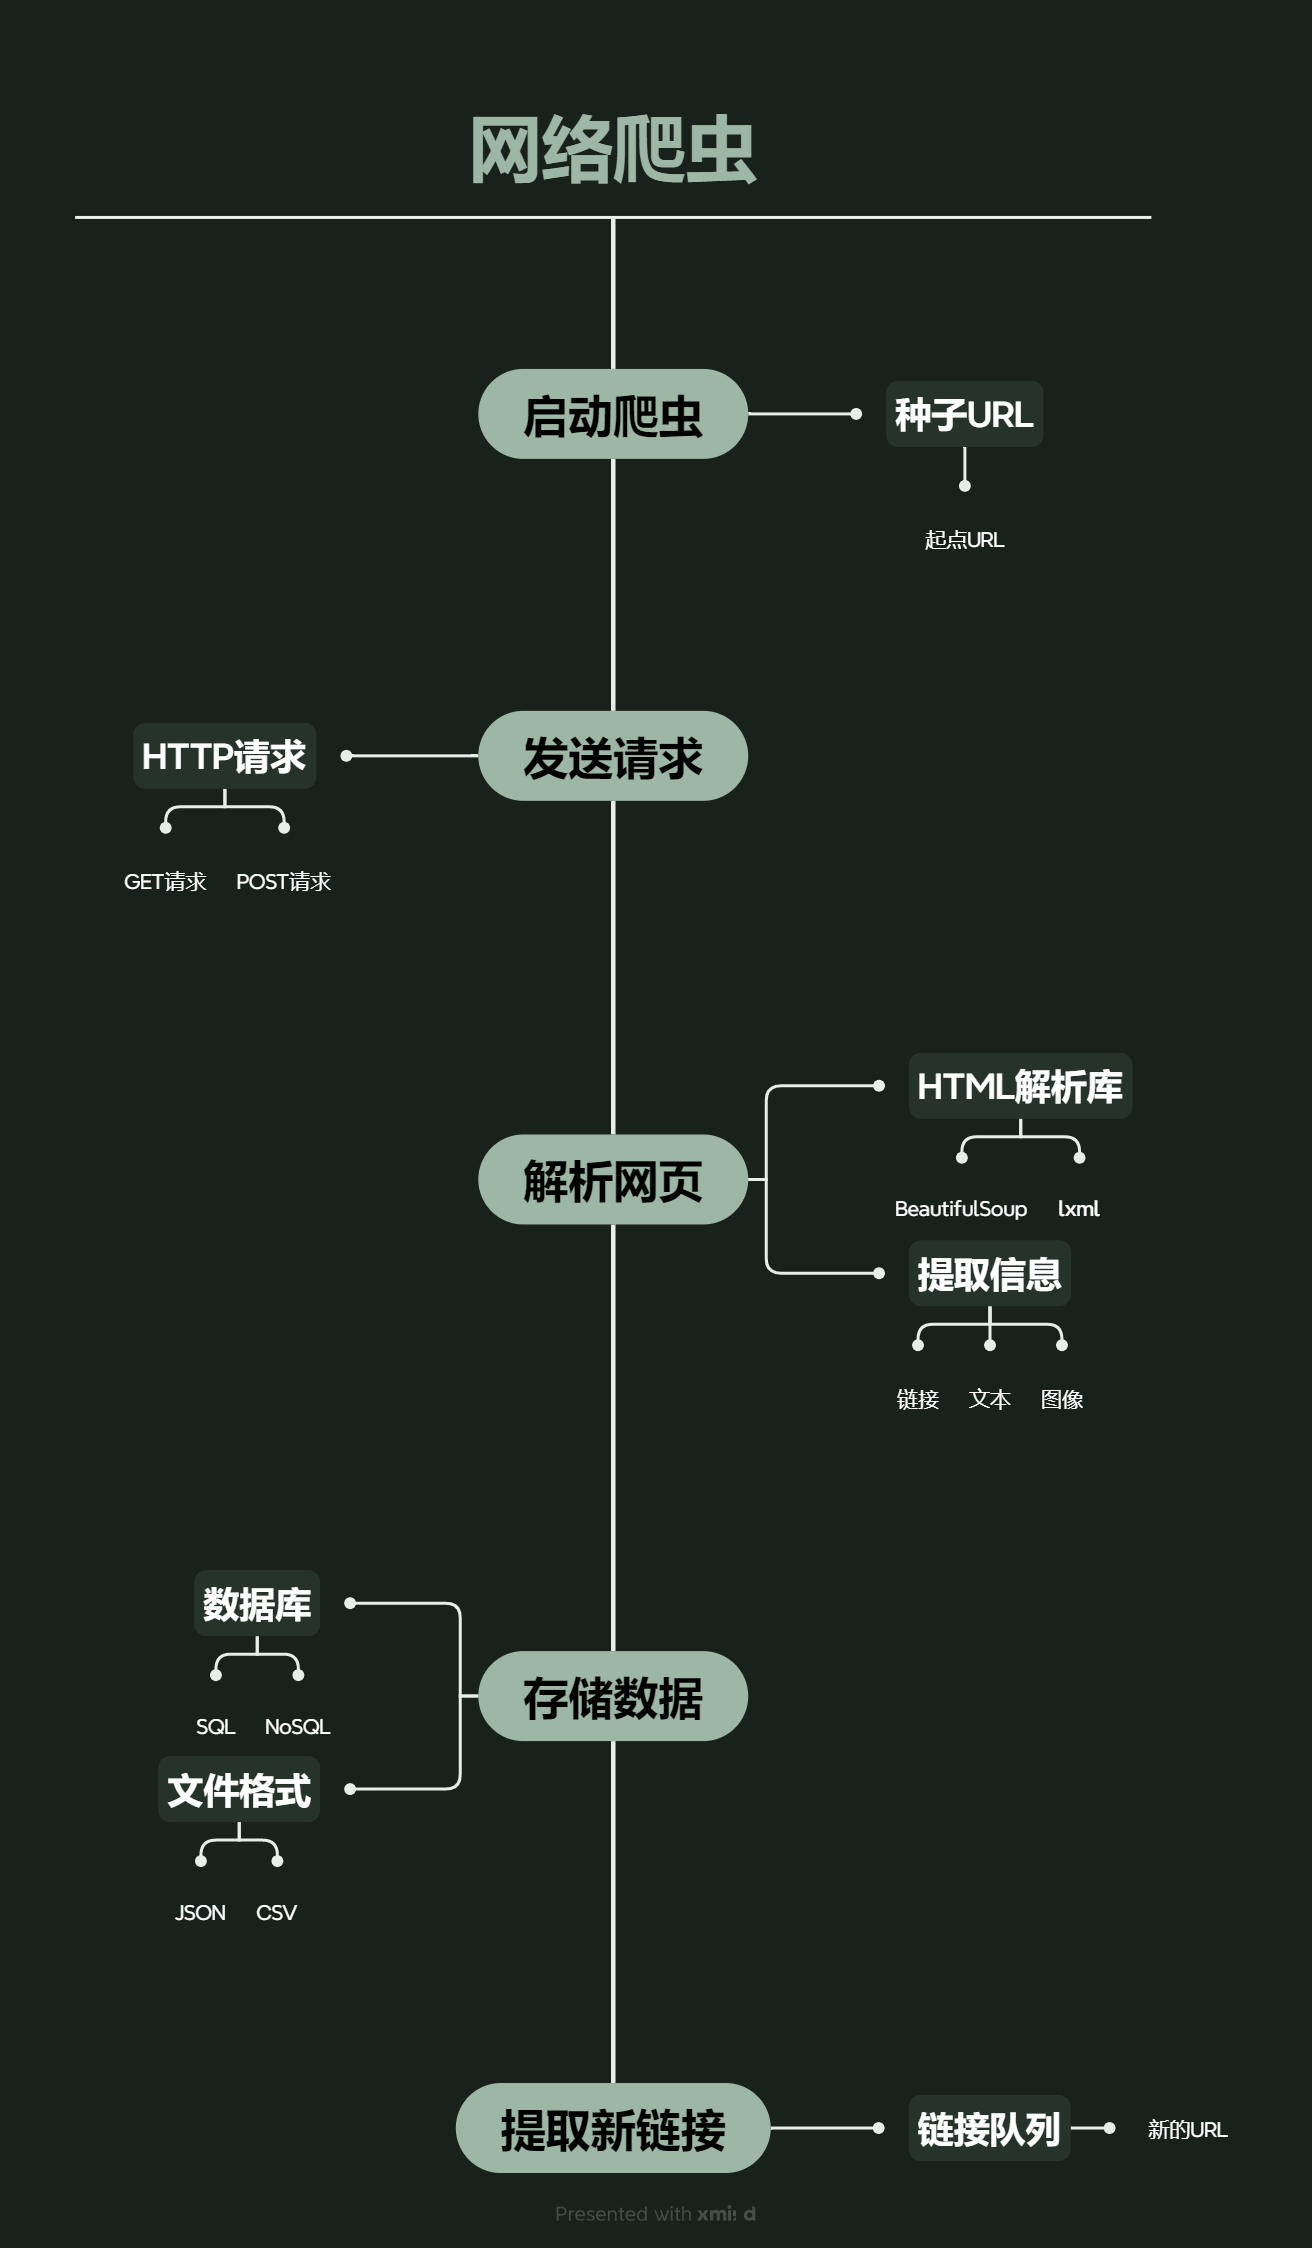
\includegraphics[width=0.5\textwidth,keepaspectratio=false]{pictures/38.png} % 修改为实际图片路径
  \caption{网络爬虫}
  
\end{figure}

\subsection{代码实现}


具体步骤包括导入库、常数定义、设计请求函数、主函数、检查重复,将在后面的实例具体讨论。
  
\section{数据处理层}

\subsection{数据预处理}

数据采集完成后,需要对其进行预处理以适配模型输入格式,因此我们有预处理阶段,旨在更好的利用数据以训练模型,达到良好的学习效果。
而前文数据爬取成狗后,数据以文本形式储存。因此,预处理阶段主要为对中文文本进行分词处理。

\subsubsection{分词作用与意义}

分词将原始的文本数据处理成计算机能够理解和处理的形式。这是自然语言处理(NLP)中的一个关键步骤,因为自然语言文本通常是一个连续的字符串,对于计算机而言,这样的形式不便于直接进行分析和处理。分词通过将文本切分成独立的词语或子词,使得文本变得结构化,更加易于进行后续的处理和分析。

分词可以显著提高文本处理的准确性和效率。将文本切分成更小的单元后,统计、查询和分析变得更加容易。这种处理方式还便于将文本转化成向量,例如词袋模型(Bag-of-Words)和词嵌入(Word Embedding)等形式,从而捕捉文本的语义信息。这种语义信息的捕捉对于提高机器学习和深度学习模型的性能非常重要,因为它能够更好地理解和解释文本内容。

\begin{figure}[H]
  \centering
  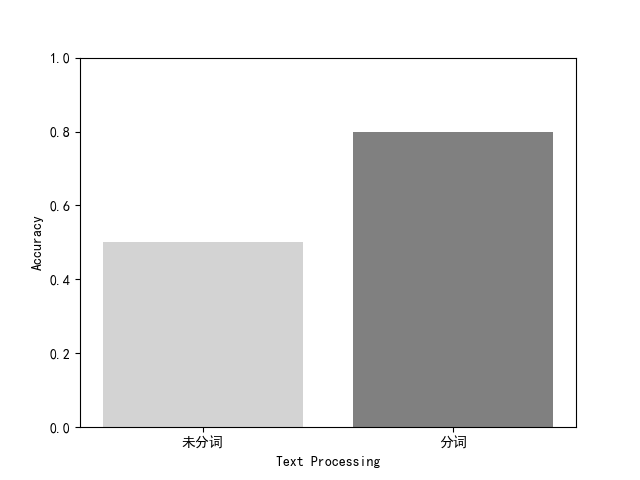
\includegraphics[width=0.5\textwidth,keepaspectratio=false]{pictures/40.png} % 修改为实际图片路径
  \caption{分词与否对模型准确度的影响}
  
\end{figure}

在情感分析等应用中,分词尤为重要。通过分词,可以识别出文本中的关键情感信息词语,这些词语对于判断文本的情感倾向至关重要。例如,分词可以将句子“我非常喜欢这款产品”分解为“我”、“非常”、“喜欢”、“这款”、“产品”,从而识别出“喜欢”这个表示积极情感的词语。这种识别可以帮助情感分析模型更加准确地判断文本的情感倾向,无论是正面、负面还是中性情感。

在数据清洗与预处理阶段,分词也发挥了重要作用。通过分词,可以去除停用词、标点符号等无关信息,使得数据更加干净整洁。停用词是指在文本处理中被过滤掉的常见词语,例如“的”、“了”、“是”等,它们通常对文本的主要内容没有贡献。去除这些停用词和无关信息后,数据变得更加简洁,模型可以更加专注于重要的信息,从而提高模型的性能。

此外,分词还可以减少文本的长度,节省计算资源,提高处理速度。在处理长文本时,分词可以将文本拆分成更小的段落或句子,便于并行处理。这种方式不仅提高了处理速度,还使得计算资源的使用更加高效。

\begin{table}[H]
  \centering
  \begin{tabular}{cc}
  \toprule
  源文本 & 分词结果\\
  \midrule
  我今天在一个美丽的花园里赏花。&	['我', '今天', '在', '一个', '美丽', '的', '花园', '里', '赏花', '。']\\
  他在书店买了一本小说。&	['他', '在', '书店', '买', '了', '一本', '小说', '。']\\
  我喜欢吃苹果和香蕉。&	['我', '喜欢', '吃', '苹果', '和', '香蕉', '。']\\
  昨天下了一场大雨。&	['昨天', '下', '了', '一场', '大雨', '。']\\
  我们一起去看电影吧。&	['我们', '一起', '去', '看', '电影', '吧', '。']\\
  \bottomrule
  \end{tabular}
  \caption{分词示例}
  \end{table}

\subsubsection{基于jieba的中文分词}

分词是自然语言处理的一个基本步骤,其目的是将一段长文本通过分词工具jieba、NLTK、spaCy等拆分成基本单元(词与子词),使得其可以作为模型输入,便于后续的工作开展。
鉴于爬虫收集的是中文文本,我们采用适用中文文本的分词工具jieba来进行分词操作。

\vskip 0.2cm
\noindent
\textbf{程序实现}

在上述代码中,我们先将jieba的日志等级设置,减少不必要的日志输出,通过正则表达式只保留爬取数据中的中文,通过正则表达式只保留爬取数据中的中文,并将剩余的字符使用word\;cut全部用空格替代以达到过滤文本的目的,
然后使用jieba进行分词操作。将get\;dataset函数用于加载数据集。最后通过调用定义的函数来实现分词的操作。

\begin{mdframed}[backgroundcolor=darkgray, linecolor=lightgray, linewidth=1pt, innermargin=0.5cm, outermargin=0.5cm, skipbelow=0.1cm]
  \color{white}
  \begin{verbatim}
  jieba.setLogLevel(logging.INFO)
  # 定义正则表达式,只保留中文字符
  regex = re.compile(r'[^\u4e00-\u9fa5]')
  \end{verbatim}
  \vspace{-1.5em} % 调整文本和底部边缘的距离
  \end{mdframed}

\subsection{关键词提取与热点分析}

在运用jieba进行分词过后,需要将以分词的文本转化为特征向量,以供机器学习。由于本次任务需要提取文本的关键词信息,
经过横向对比分析,为了实现识别文本中的主体并综合分析多个文本以提取热点词语,TF-IDF特征提取是最佳选择。
这种方法可以捕捉词的全局重要性,从而更准确地提取文本中的关键主体和热点词语。

\subsubsection{TF-IDF特征提取}

TF-IDF是一种用于文本特征提取的方法,它结合了词频(TF)和逆文档频率(IDF)来衡量词的重要性。

\vskip 0.2cm
\noindent
\textbf{TF(词频)}

词频衡量一个词在文档中出现的频率。对于一个给定的词$t$和文档$d$,词频的计算公式为:

\begin{equation}
  \text{TF}(t, d) = \frac{\text{出现次数}(t, d)}{\text{文档}\, d\, \text{中的总词数}}
\end{equation}

\vskip 0.2cm
\noindent
\textbf{IDF(逆文档频率)}

逆文档频率衡量一个词在整个文档集中的重要性。对于一个给定的词 \( t \) 和文档集 \( D \),逆文档频率的计算公式为:

\begin{equation}
\text{IDF}(t, D) = \log \frac{N}{1 + |\{d \in D : t \in d\}|}
\end{equation}

其中,$N$是文档集中文档的总数。
$|\{d \in D : t \in d\}|$是包含词$t$的文档数量。

\vskip 0.2cm
\noindent
\textbf{TF-IDF}

TF-IDF 是 TF 和 IDF 的乘积,用来衡量词 $t$ 在文档 $d$ 中的重要性:

\begin{equation}
\text{TF-IDF}(t, d, D) = \text{TF}(t, d) \times \text{IDF}(t, D)
\end{equation}

由于jieba分词过后得到了中文语境的文段分词,TF-IDF特征提取结果便是一段文本
的每个分词的重要性特征向量。通过此特征向量可以很好概括各词重要性。
在此我们运用几个示例展示TF-IDF计算词汇重要性的结果:

采用以下案例:
\begin{table}[H]
  \centering
  \begin{tabular}{cc}
  \toprule
  标号 & 文本\\
  \midrule
  1 & "我喜欢吃苹果"\\
  2 & "我喜欢吃香蕉"\\
  3 & "我不喜欢吃苹果"\\
  4 & "他喜欢吃苹果"\\
  5 & "我和他都喜欢吃苹果"\\
  \bottomrule
  \end{tabular}
  \caption{示例文本}
  \end{table}

对此五句示例文本应用TF-IDF特征提取,得到各词的重要性指数,嵌入至该文本的特征向量,绘制以下热图:

  \begin{figure}[H]
    \centering
    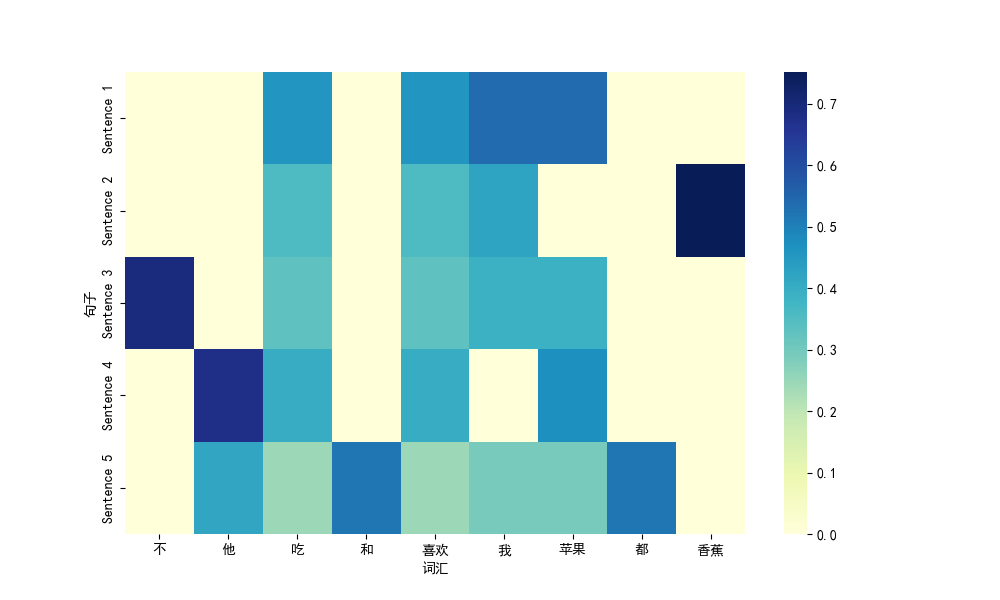
\includegraphics[width=0.8\textwidth,keepaspectratio=false]{pictures/1.png} % 修改为实际图片路径
    \caption{示例文本在TF-IDF方法下的特征提取结果}
    
  \end{figure}

  \begin{table}[H]
    \centering
    \begin{tabular}{cccccccccc}
    \toprule
    文本标号&不&他&吃&和&喜欢&我&苹果&都&香蕉\\
    \midrule
    1 & [0.000000 & 0.000000 & 0.456637 & 0.000000 & 0.456637 & 0.539892 & 0.539892 & 0.000000 & 0.000000]\\
    2 & [0.000000 & 0.000000 & 0.358010 & 0.000000 & 0.358010 & 0.423283 & 0.000000 & 0.000000 & 0.751325]\\
    3 & [0.691894 & 0.000000 & 0.329691 & 0.000000 & 0.329691 & 0.389801 & 0.389801 & 0.000000 & 0.000000]\\
    4 & [0.000000 & 0.676468 & 0.399533 & 0.000000 & 0.399533 & 0.000000 & 0.472376 & 0.000000 & 0.000000]\\
    5 & [0.000000 & 0.417193 & 0.246401 & 0.517099 & 0.246401 & 0.291325 & 0.291325 & 0.517099 & 0.000000]\\
    \bottomrule
    \end{tabular}
    \caption{示例文本TF-IDF特征提取向量}
    \end{table}

可以看到,TF-IDF基于各词重要性很好的提取了文本信息。

\subsubsection{热点识别}

文本经过TF-IDF处理后,可以很好的得到各词汇重要性分布。从而,在输入大量数据后,可以得到某领域舆论的最新热点词汇。

本次实验采用某地区投诉意见文本数据集,具体数据展示如下:

\lstinputlisting{train_hot_word.txt}

针对该数据集应用TF-IDF方法进行热点分析,并从中选取排名前50的词汇进行分析。获取不同词汇的重要性指数,绘制云图如下:

\begin{figure}[H]
  \centering
  
\includegraphics[width=0.7\textwidth,keepaspectratio=false]{pictures/11.png} % 修改为实际图片路径
  \caption{实验数据的热点词汇云图}
\end{figure}

将各词汇重要性进行统计:

\begin{figure}[H]
  \centering
  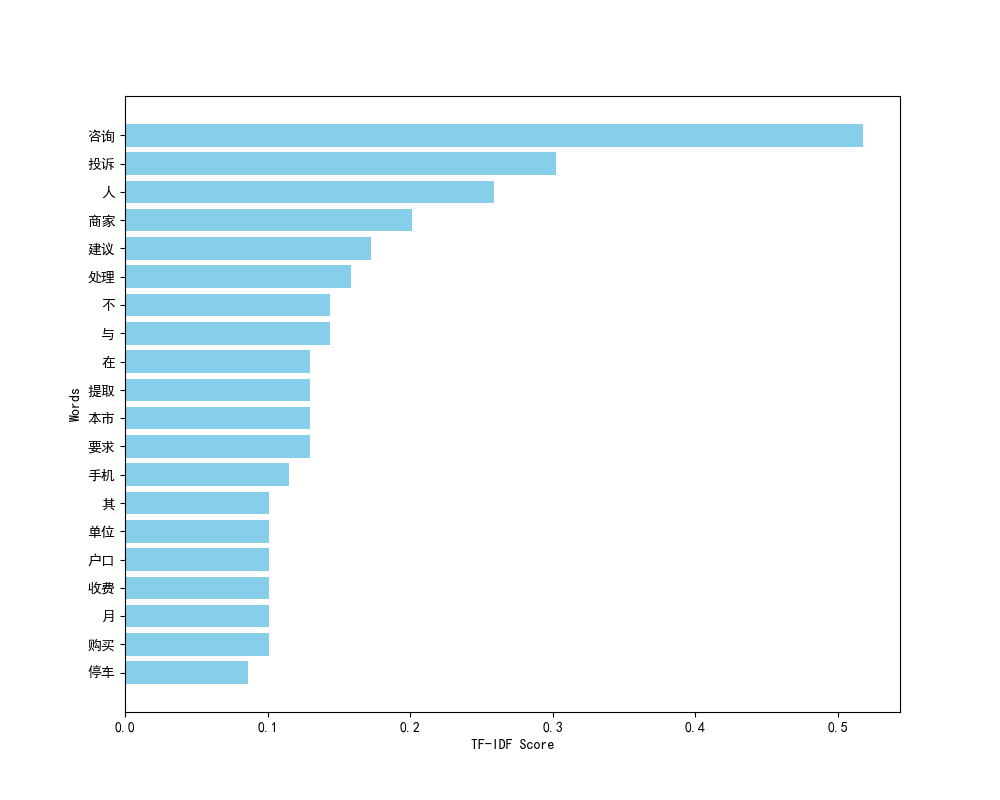
\includegraphics[width=0.5\textwidth,keepaspectratio=false]{pictures/12.png} % 修改为实际图片路径
  \caption{各热点词汇重要性指数统计}
\end{figure}

可以看到,此数据集因为是投诉建议为主,所以热点词汇为咨询、投诉、商家等。由此可见,我们的模型是准确可靠的。

\subsubsection{热点趋势分析}

TF-IDF已经得出了各词在语段中的重要性,通过排序可以得到语段中的词语热点排名。然而,若要进行趋势分析,需要引入预测模型
进行热点趋势预测。

时间序列预测模型主要用于分析和预测随时间变化的数据点。这些模型试图捕捉数据中的趋势、季节性模式和噪声,
从而对未来的数据点进行预测。其中一个广泛使用的时间序列预测模型是 ARIMA,即自回归积分滑动平均模型。

\vskip 0.2cm
\noindent
\textbf{ARIMA时间序列预测模型构建}

ARIMA 模型是时间序列预测中的一种经典方法,用于理解单变量时间序列数据集并预测未来点。
它结合了三个基本概念:自回归(AR)、差分(I)和移动平均(MA)。

\vskip 0.2cm
\noindent
\textbf{1. 自回归部分 (AR)}

自回归部分定义了观测值与其若干滞后观测值之间的关系:

\begin{equation}
X_t = c + \phi_1 X_{t-1} + \phi_2 X_{t-2} + \cdots + \phi_p X_{t-p} + \epsilon_t
\end{equation}

其中,$X_t$ 是时间 $t$ 的时间序列值,$c$ 是常数,$\phi_1, \phi_2, \ldots, \phi_p$ 是模型参数,$\epsilon_t$ 是白噪声。

\vskip 0.2cm
\noindent
\textbf{2. 差分部分 (I)}

差分部分用于通过从当前观测值中减去前一观测值使时间序列变得平稳:

\begin{equation}
\Delta X_t = X_t - X_{t-1}
\end{equation}

此操作执行 $d$ 次以达到平稳状态。

\vskip 0.2cm
\noindent
\textbf{3. 移动平均部分 (MA)}

移动平均部分模型描述了观测值与应用于滞后观测值的移动平均模型的残差误差之间的关系:

\begin{equation}
X_t = \mu + \epsilon_t + \theta_1 \epsilon_{t-1} + \theta_2 \epsilon_{t-2} + \cdots + \theta_q \epsilon_{t-q}
\end{equation}

其中,$\mu$ 是序列的平均值,$\theta_1, \theta_2, \ldots, \theta_q$ 是模型参数,$\epsilon_t$ 是误差项。

\vskip 0.2cm
\noindent
\textbf{组合 ARIMA 模型}

结合上述所有组成部分,ARIMA(p, d, q) 模型可以表示为:

\begin{equation}
(1 - \phi_1 B - \phi_2 B^2 - \cdots - \phi_p B^p)(1 - B)^d X_t = (1 + \theta_1 B + \theta_2 B^2 + \cdots + \theta_q B^q) \epsilon_t
\end{equation}

其中 $B$ 是回退(或延迟)算子。如果 $X_t$ 是当前值,那么 $BX_t = X_{t-1}$。

\vskip 0.2cm
\noindent
\textbf{模型测试}

由于预测模型所需的数据量极大,本次实验采用酒店评论数据集,共包含5000条评论信息。

\begin{figure}[H]
  \centering
  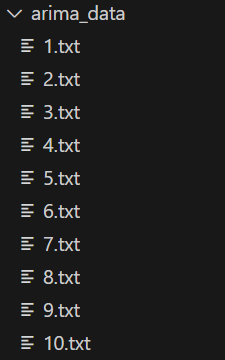
\includegraphics[width=0.2\textwidth,keepaspectratio=false]{pictures/21.png} % 修改为实际图片路径
  \caption{实验数据集}
\end{figure}

本次预测模型的测试将原先的大数据集分为十个小数据集,分别作为十个时间点的源数据,进行后续时间点的热点词汇预测。

应用ARIMA模型后,可以得到各热点词汇变化趋势如下:

\begin{figure}[H]
  \centering
  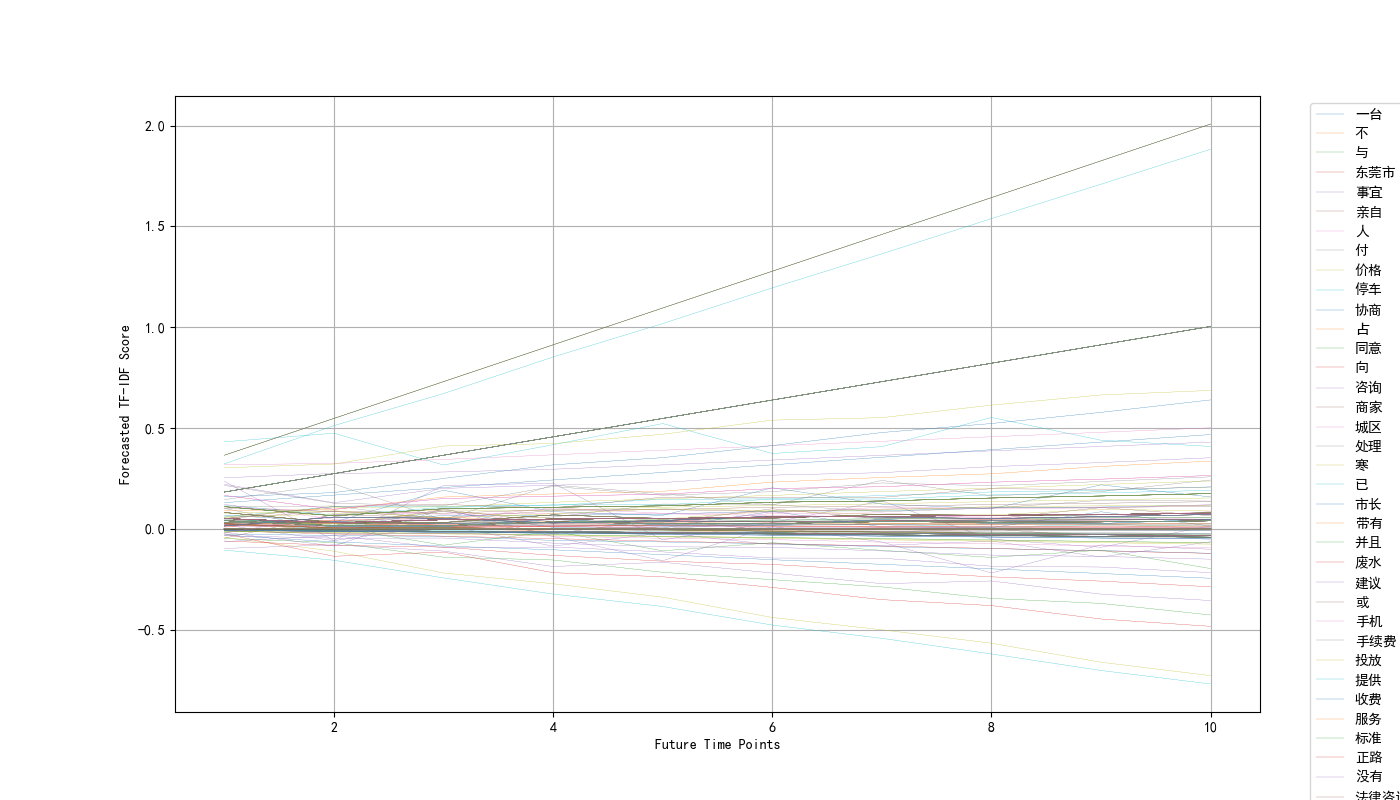
\includegraphics[width=0.7\textwidth,keepaspectratio=false]{pictures/13.png} % 修改为实际图片路径
  \caption{各热点词汇趋势预测}
\end{figure}

取未来六个时间点的各词汇重要性指数绘制热词云图,如下所示:

\begin{figure}[htbp]
  \centering
  
  \begin{subfigure}{0.32\textwidth}
    
\includegraphics[width=\linewidth]{pictures/14.png}
    \caption{时间点1}
  \end{subfigure}
   % 添加空白以分隔子图
  \begin{subfigure}{0.32\textwidth}
    
\includegraphics[width=\linewidth]{pictures/15.png}
    \caption{时间点2}
  \end{subfigure}
  \hfill
  \begin{subfigure}{0.32\textwidth}
    
\includegraphics[width=\linewidth]{pictures/16.png}
    \caption{时间点3}
  \end{subfigure}
  
  \vspace{0.2em} % 在行之间添加一些额外的空间
  
  \begin{subfigure}{0.32\textwidth}
    
\includegraphics[width=\linewidth]{pictures/17.png}
    \caption{时间点4}
  \end{subfigure}
  \hfill
  \begin{subfigure}{0.32\textwidth}
    
\includegraphics[width=\linewidth]{pictures/18.png}
    \caption{时间点5}
  \end{subfigure}
  \hfill
  \begin{subfigure}{0.32\textwidth}
    
\includegraphics[width=\linewidth]{pictures/19.png}
    \caption{时间点6}
  \end{subfigure}
  
  \caption{未来多时间节点预测云图}
  \end{figure}

可以看到,预测序列值稳定可靠,预测结果中"酒店"、"房间"等词重要性较高稍有波动,符合实际情况与常识,
说明模型是普适、实用的。

\section{分析层}

\subsection{主题模型}

在舆论分析中,主题分析(或称话题分析)扮演着核心角色,特别是在理解公众讨论的广泛问题或焦点时。这项技术通过从大量文本数据中提取有意义的信息来帮助我们洞察群众的观点内容与导向。
此过程涉及对一段给定文本进行特征提取后,利用主体模型分析其所表达的主要意图与文本主题。

在训练机器以提取文本主题过程中有两种方式,一种为有监督学习,即预先准备带有标签的数据集训练分类器,还有一种则是无监督学习,即识别文本的潜在主题分布。
首先我们考虑第一种主题分析方法。


第一种方式,需要准备文本材料即对应的主题标签,随后对文本进行特征提取,进而训练分类器使得特征与类别正确匹配。
由于在分析文本主题的过程中,需要同时考虑分词重要性与文本上下文,因此TF-IDF特征提取结合BERT嵌入的文本特征提取方式是最佳选择
上文已经论述TF-IDF提取方式的具体应用,因此此处主要讨论BERT嵌入方式的原理即应用。

\subsubsection{BERT嵌入}

BERT(Bidirectional Encoder Representations from Transformers)
是一种预训练的深度学习模型,主要用于自然语言处理任务。BERT的核心是Transformer的编码器架构,
这是一种依靠自注意力机制处理序列数据的方法。

\vskip 0.2cm
\noindent
\textbf{方法原理}

BERT的关键特点是其双向性,即模型同时考虑序列中每个词之前和之后的所有词。
这种全方位的上下文理解显著提升了模型对语言的理解能力。

BERT的训练包括两个主要任务:
\textbf{Masked Language Model (MLM)},随机遮蔽输入句子中的某些词(例如将它们替换为一个特殊的[MASK]标记),然后模型需要预测这些遮蔽词。
\textbf{Next Sentence Prediction (NSP)},给定两个句子A和B,模型需要预测B是否是A的下一句。


\vskip 0.2cm
\noindent
\textbf{自注意力机制}

自注意力是BERT中的关键组件,它使模型能够根据句子中的其他词加权重视当前词。
对于输入序列 \(X = (x_1, x_2, \ldots, x_n)\),自注意力的输出计算如下:

首先,计算查询(Q)、键(K)和值(V):

\begin{equation}
Q = XW^Q, \quad K = XW^K, \quad V = XW^V
\end{equation}

这里 \(W^Q\), \(W^K\), \(W^V\) 是可学习的权重矩阵。

随后计算计算注意力分数:

\begin{equation}
\text{Attention}(Q, K, V) = \text{softmax}\left(\frac{QK^T}{\sqrt{d_k}}\right)V
\end{equation}

其中 \(d_k\) 是键向量的维度,这个除法操作是为了保持数值的稳定性。

\vskip 0.2cm
\noindent
\textbf{实例应用}

依然考虑TF-IDF特征提取示例中五个相似句子,我们采用BERT方法进行特征向量的提取。由于BERT特征提取一般是高维的,本次采用t-SNS降维使得
各提取的特征向量二维可视化,如下图所示:

\begin{figure}[H]
  \centering
  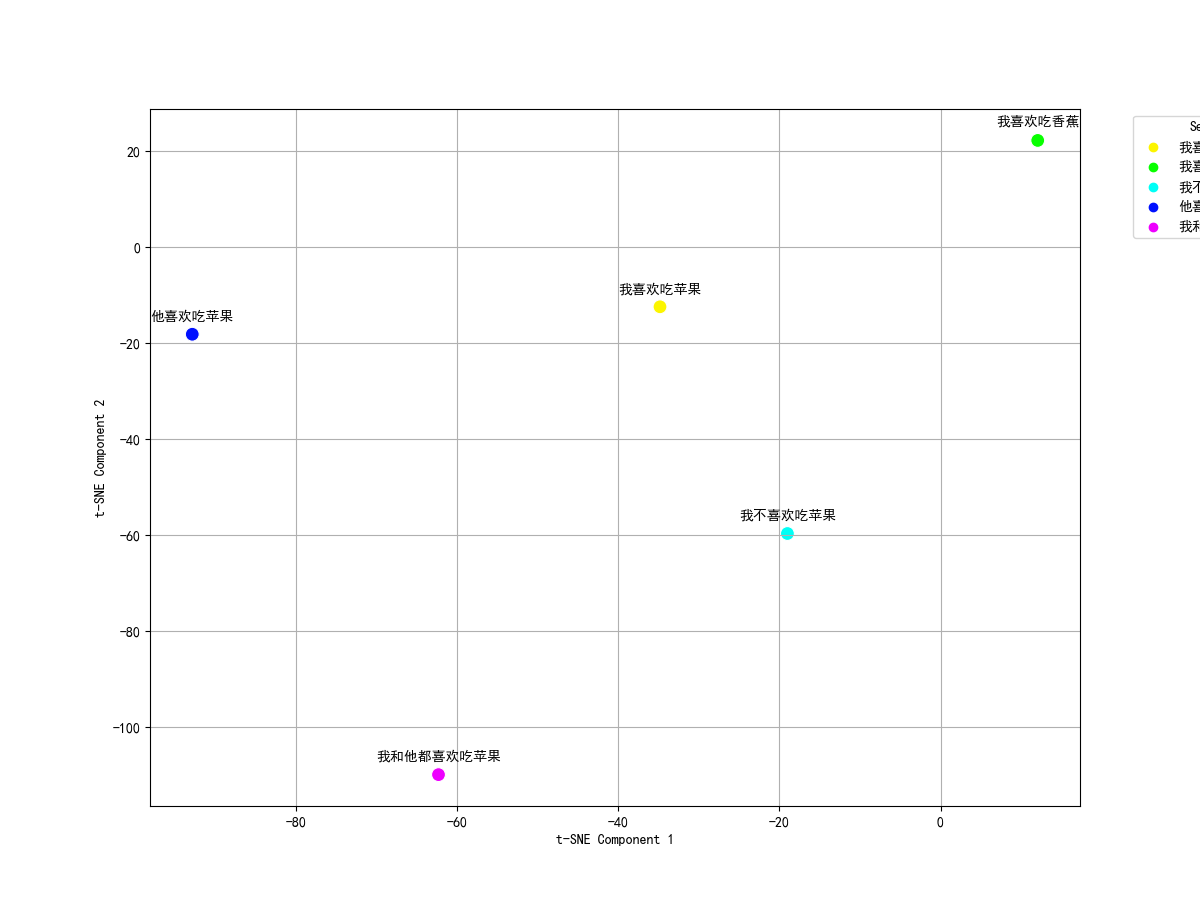
\includegraphics[width=0.6\textwidth,keepaspectratio=false]{pictures/2.png} % 修改为实际图片路径
  \caption{示例文本在BERT方法下的特征提取经t-SNS降维后结果}
  \label{2}
\end{figure}

随后,调出BERT方法应用过程中的注意力图,可以看到各字权重(BERT不采用jieba分词,以单字为单位):

\begin{figure}[H]
  \centering
  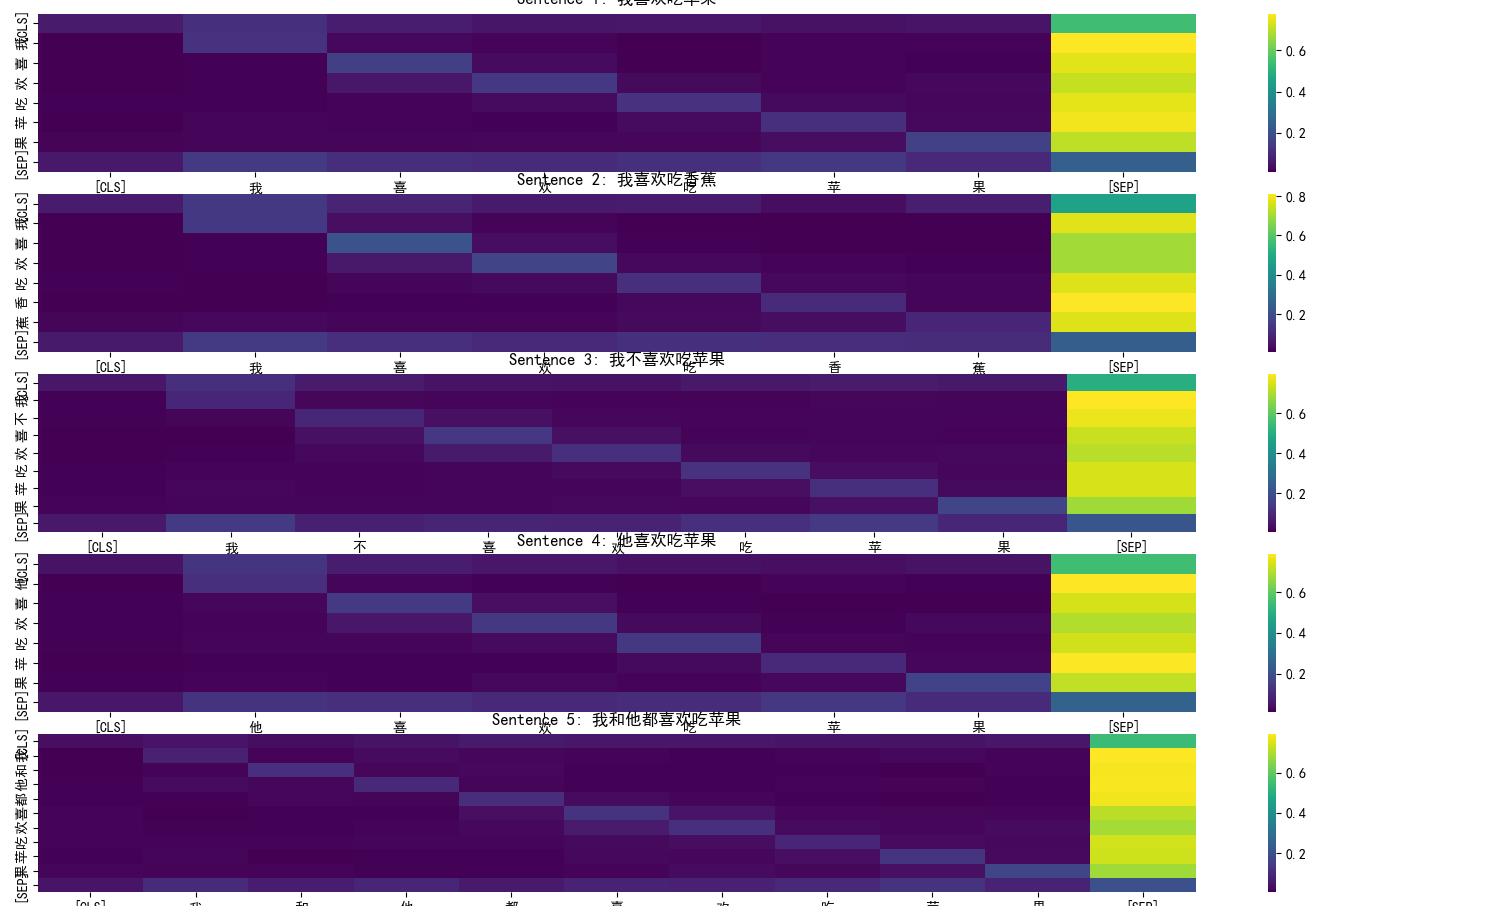
\includegraphics[width=0.6\textwidth,keepaspectratio=false]{pictures/3.png} % 修改为实际图片路径
  \caption{各文本在BERT方法下各字注意力权重图}
  
\end{figure}

可以看到,BERT方法处理下,各词之间的关联信息被很好提取。

\subsubsection{特征整合}

在分别进行TF-IDF特征提取处理与BERT嵌入处理后,由于特征向量的维度不同,而又需同时考虑字词相互联系、重要性,
于是采用串联(Concatenation),同时利用BERT的深度上下文理解能力和TF-IDF的关键词统计信息,从而提供更丰富和综合的文本表示。

假设对于一个给定的文本 \( T \),我们已经得到:
BERT特征向量 \( \vec{v}_{\text{BERT}} \)
和TF-IDF特征向量 \( \vec{v}_{\text{TF-IDF}} \),
两种特征向量的整合可以通过向量串联实现,具体公式如下:

\begin{equation}
\vec{v}_{\text{combined}} = \left[ \vec{v}_{\text{BERT}}; \vec{v}_{\text{TF-IDF}} \right]
\end{equation}

这里的 \( ; \) 表示向量的串联。

\subsubsection{有监督学习主题模型}

\vskip 0.2cm
\noindent
\textbf{模型原理}

在进行特征提取后,需要建立有监督学习主题模型以识别文本主题,采用朴素贝叶斯分类器方法进行分类训练,可以很好的达到
精准识别主题的目的。


朴素贝叶斯分类器是一种简单而有效的机器学习算法,特别适用于文本分类问题。
朴素贝叶斯分类器基于贝叶斯定理,并假设特征之间相互独立:
\begin{equation}
  P(A|B) = \frac{P(B|A) \cdot P(A)}{P(B)}
  \end{equation}
  
  其中,\(P(A|B)\) 是在知道 \(B\) 发生的情况下 \(A\) 发生的概率,
\(P(B|A)\) 是在知道 \(A\) 发生的情况下 \(B\) 发生的概率,
\(P(A)\) 是 \(A\) 发生的先验概率,
\(P(B)\) 是 \(B\) 发生的先验概率。


此次分类问题中,目标是计算在给定样本特征向量 \(\mathbf{x}=[x_1, x_2, \ldots, x_n]\) 时,每个类别 \(C_k\) 的后验概率 \(P(C_k|x_1, x_2, \ldots, x_n)\),然后选择概率最大的类别。公式如下:

\begin{equation}
P(C_k|x_1, x_2, \ldots, x_n) \propto P(C_k) \prod_{i=1}^{n} P(x_i|C_k)
\end{equation}

朴素贝叶斯模型中多项式朴素贝叶斯(MultinomialNB)是常见变体,适用于特征是计数数据的情况。
其条件概率计算公式为:

\begin{equation}
P(x_i|C_k) = \frac{N_{C_k, x_i} + \alpha}{N_{C_k} + \alpha \cdot n}
\end{equation}

其中,
\(N_{C_k, x_i}\) 是在类别 \(C_k\) 中特征 \(x_i\) 出现的次数,
\(N_{C_k}\) 是在类别 \(C_k\) 中所有特征出现的总次数,
\(n\) 是特征的总数,
\(\alpha\) 是平滑参数(通常取1,称为拉普拉斯平滑)。

\vskip 0.2cm
\noindent
\textbf{模型测试}

本次进行有监督主题模型测试的数据集为日常作息文本数据,附带8个标签,如下表所示:

\begin{table}[H]
  \centering
  \begin{tabular}{ccc}
  \toprule
  标签&数据量&示例\\
  \midrule
  吃饭 & 200&"我想吃火锅"\\
  睡觉 & 200&"今天熬个夜吧"\\
  写作业 &200&"作业好难,写不完了"\\
  锻炼 & 200&"今天去健身房"\\
  编程 & 200&"正在写一个Python脚本"\\
  出游 & 200&"下个月去旅游"\\
  谈恋爱 & 200&"和女朋友逛街"\\
  写论文 & 200&"写一篇关于人工智能的论文"\\
  
  \bottomrule
  \end{tabular}
  \caption{示例数据}
  \end{table}

经过模型训练后,我们得到测试数据的混淆矩阵如下所示:

\begin{figure}[H]
  \centering
  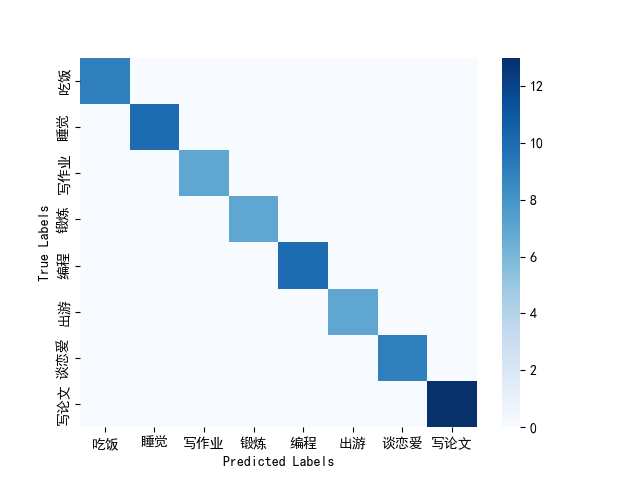
\includegraphics[width=0.7\textwidth,keepaspectratio=false]{pictures/23.png} % 修改为实际图片路径
  \caption{有监督主题模型测试混淆矩阵}
  
\end{figure}

可以看到,正确率(accuracy)为1.0,模型测试准确度极高。

绘制测试的ROC曲线及召回率曲线:

\begin{figure}[H]
  \centering
  \centering
  
  \begin{subfigure}{0.45\textwidth}
    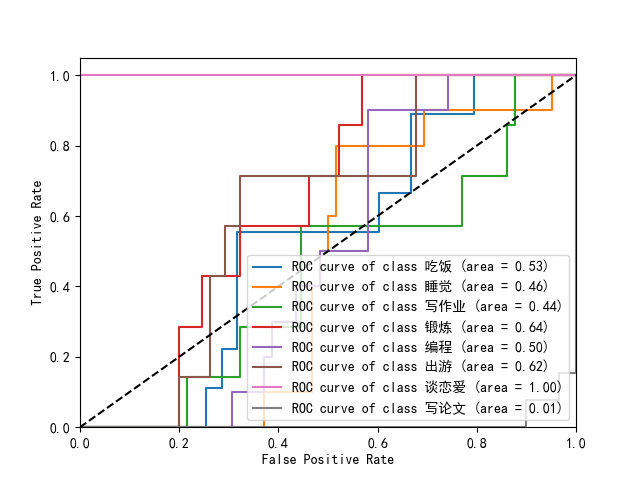
\includegraphics[width=\linewidth]{pictures/24.png}
    \caption{ROC曲线}
  \end{subfigure}
   % 添加空白以分隔子图
  \begin{subfigure}{0.45\textwidth}
    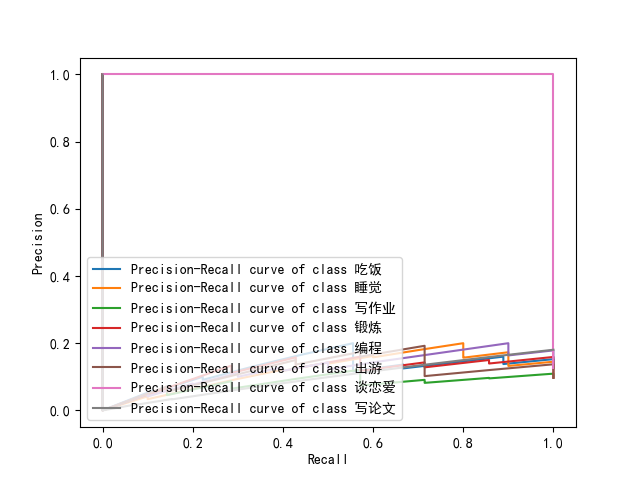
\includegraphics[width=\linewidth]{pictures/25.png}
    \caption{精确-召回率}
  \end{subfigure}
  
\end{figure}

由此可见,我们的模型是可靠的、稳定的,具有极高的准确度、普适性。

应用模型,可以得到下列三条示例文本的测试结果:

\begin{table}[H]
  \centering
  \begin{tabular}{cc}
  \toprule
  测试文本&标签结果\\
  \midrule
  焦虑的只想睡觉 & 睡觉\\
  我写论文写的想死 & 写论文\\
  我是一个程序猿 &编程\\

  \bottomrule
  \end{tabular}
  \caption{测试结果}
  \end{table}


  测试结果符合实际,因此,我们的模型可以后续被应用到实际的舆情主题分析中。

\subsubsection{潜在主题模型}

LDA(Latent Dirichlet Allocation,潜在狄利克雷分配)
是一种广泛应用于自然语言处理和文档分析的主题模型。
它是由Blei, Ng, 和Jordan在2003年提出的,用于从文档集合中自动发现文档中的主题。
LDA 是一个生成模型,它假设文档是由隐含的主题构成,而这些主题则决定了文档中的单词分布。

\vskip 0.2cm
\noindent
\textbf{基本原理}

狄利克雷分配是一种连续概率分布,通常用于生成一组概率分布的先验分布。其概率密度函数定义如下:

\begin{equation}
p(\theta | \alpha) = \frac{1}{B(\alpha)} \prod_{i=1}^K \theta_i^{\alpha_i - 1}
\end{equation}

其中,\(\theta\) 是一个 \(K\) 维的概率向量,每个 \(\theta_i\) 满足 \(0 \leq \theta_i \leq 1\) 且 \(\sum_{i=1}^K \theta_i = 1\)。
\(\alpha\) 是一个 \(K\) 维的参数向量,每个 \(\alpha_i > 0\)。
\(B(\alpha)\) 是狄利克雷分布的标准化常数,称为贝塔函数:
\begin{equation}
    B(\alpha) = \frac{\prod_{i=1}^K \Gamma(\alpha_i)}{\Gamma\left(\sum_{i=1}^K \alpha_i\right)}
  \end{equation}

LDA 假设文档生成的过程遵循以下步骤:

1. 选择文档的主题分布:对于每篇文档,选择一个主题分布。这个分布是从一个狄利克雷分布中采样得到的。狄利克雷分布是一个连续多元概率分布,非常适合表达多项分布的共轭先验。

2. 生成文档中的每个词:

选择一个主题:对于文档中的每个词,首先根据文档的主题分布选择一个主题。

选择一个词:然后,根据所选主题的词分布,从该主题对应的多项分布中选择一个词。这个多项分布定义了每个主题下词的概率。

\vskip 0.2cm
\noindent
\textbf{数学模型}

选择 $N \sim \text{Poisson}(\xi)$,即文档中的词数。

选择 $\theta \sim \text{Dirichlet}(\alpha)$,即文档的主题分布。

对于文档中的每个词 $w_n$:
    
        \;\;\;\;\;\;\;\;选择一个主题 $z_n \sim \text{Multinomial}(\theta)$。

        \;\;\;\;\;\;\;\;根据主题 $z_n$ 从条件多项分布 $p(w_n | z_n, \beta)$ 中选择一个词 $w_n$。

\begin{figure}[H]
  \centering
  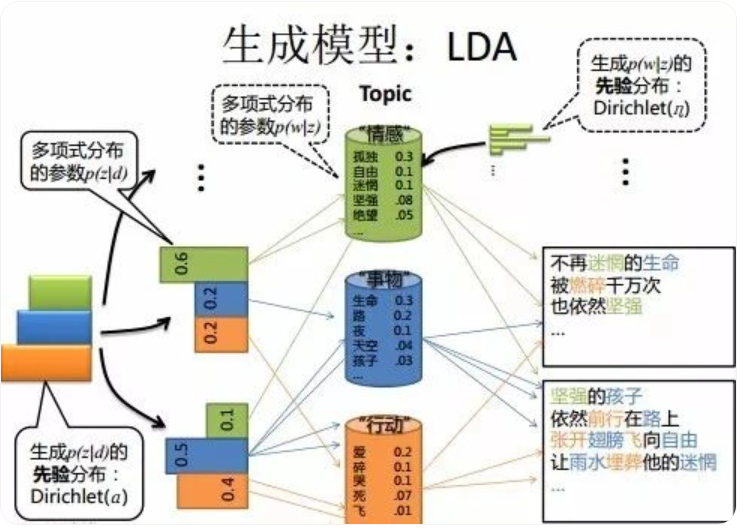
\includegraphics[width=0.6\textwidth,keepaspectratio=false]{pictures/36.png} % 修改为实际图片路径
  \caption{LDA主题模型架构}
  
\end{figure}

\subsubsection{模型测试}

在构建完LDA模型后,采用原先的热点分析中所用到的酒店评论数据集作为本次测试数据集。应用LDA,可以得到所有文本
提炼出的五个潜在主题:

\begin{table}[H]
  \centering
  \begin{tabular}{cc}
  \toprule
  潜在主题&词汇贡献\\
  \midrule
  1 & 0.003*"酒店" + 0.002*"是" + 0.002*"我" + 0.001*"房间" + 0.001*"很" \\
  2 & 0.024*"酒店" + 0.022*"是" + 0.018*"很" + 0.017*"房间" + 0.016*"我"\\
  3 &0.002*"我" + 0.001*"房间" + 0.001*"是" + 0.001*"酒店" + 0.001*"很"\\
  4 &0.021*"是" + 0.021*"酒店" + 0.017*"我" + 0.015*"房间" + 0.008*"不"\\
  5 &0.012*"酒店" + 0.011*"是" + 0.011*"我" + 0.008*"不" + 0.007*"说"\\
  \bottomrule
  \end{tabular}
  \caption{测试结果}
  \end{table}

  此处列出了排名前五的词汇贡献,通过分析,可以将此五个主题依次解释为:酒店总体评价、房间和服务的评价、
  住宿体验和位置相关、房间设施和整体环境、其他方面。

  绘制五个潜在主题云图,如下所示:

  \begin{figure}[htbp]
    \centering
    
    \begin{subfigure}{0.32\textwidth}
      
\includegraphics[width=\linewidth]{pictures/26.png}
      \caption{主题1}
    \end{subfigure}
     % 添加空白以分隔子图
    \begin{subfigure}{0.32\textwidth}
      
\includegraphics[width=\linewidth]{pictures/27.png}
      \caption{主题2}
    \end{subfigure}
    \hfill
    \begin{subfigure}{0.32\textwidth}
      
\includegraphics[width=\linewidth]{pictures/28.png}
      \caption{主题3}
    \end{subfigure}
    \vspace{0.2em} % 在行之间添加一些额外的空间
    

    \begin{subfigure}{0.32\textwidth}
      
\includegraphics[width=\linewidth]{pictures/29.png}
      \caption{主题4}
    \end{subfigure}
    \hspace{0.2cm}
    \begin{subfigure}{0.32\textwidth}
      
\includegraphics[width=\linewidth]{pictures/30.png}
      \caption{主题5}
    \end{subfigure}
    
    \caption{每个潜在主题的词汇贡献云图}
    \end{figure}

    在解释完成每个潜在主题后,便可通过每个主题对特定文本的贡献,得出文本的最终主题,绘制如下柱状图:

    \begin{figure}[H]
      \centering
      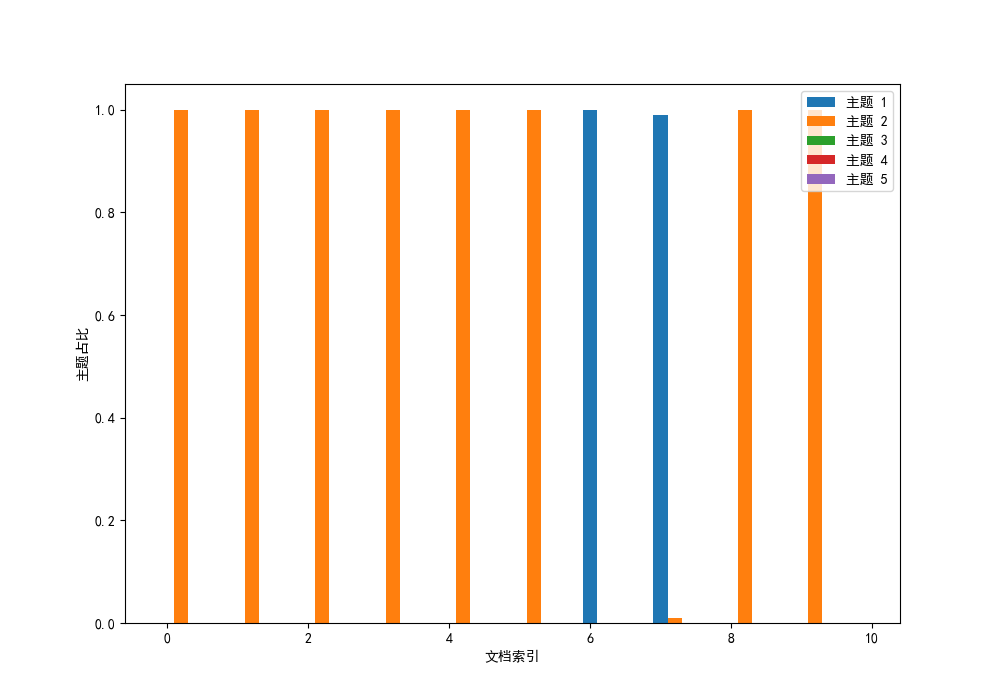
\includegraphics[width=0.6\textwidth,keepaspectratio=false]{pictures/31.png} % 修改为实际图片路径
      \caption{各文本潜在主题}
      
    \end{figure}

  由图可知,6、7文本语段主要意义为房间和服务的评价,其他语段主要为酒店总体评价。

综上,通过潜在主题的识别、解释、计算贡献,便可以得到各输入文本的潜在主题内核,从而分析当今热门话题含义。


\subsection{情感分析}

智能舆情分析应用中的情感分析模块旨在识别文本的情感倾向(正面、负面、中性),
并进一步分析情感的强度。进行基于深度学习的情感分类,首先要对语句进行分词、停用词、简繁转换等预处理,
然后进行词向量编码,然后利用LSTM或者GRU等RNN网络进行特征提取,
最后通过全连接层和softmax输出每个分类的概率,从而得到情感分类。

前文已论述如何进行数据预处理,包括分词、停用词过滤、简繁转换等。
此过程中,需要确保文本中的噪声和无关信息最小化,提升后续模型的准确性。由于
情感分许与热点分析、主题分析的差异性,与文本特征提取部分,重新进行方法选择。

\subsubsection{文本特征提取}

我们需要实现的功能是:将文本转换为向量,以便输入到深度学习模型中。
期间,需要重点考虑如何选择合适的词向量库,处理特定场景下的缺失词向量。

我们按以下步骤处理文本:

\vskip 0.2cm
\noindent
\textbf{加载词向量}

加载预训练的词向量(如Word2Vec, GloVe),并结合特定场景的增量训练。网上下载的词向量获取简单,往往缺失特定场景的词语。比如大众点评菜品场景下的鱼香肉丝、干锅花菜等词语。而自己训练则需要大量的语料,训练时间长,成本较高。所以将两种方法结合。

\vskip 0.2cm
\noindent
\textbf{建立词语到词向量的映射}

将文本中的词语映射到对应的词向量,并创建一个词向量矩阵以供模型使用。使用Keras的Tokenizer来建立词语索引,并创建一个词向量矩阵,词向量矩阵的每一行表示一个词语的词向量。矩阵的行数等于词汇表的大小加1(考虑到索引从1开始)。

\vskip 0.2cm
\noindent
\textbf{编码文本}

使用嵌入层将文本中的词语转换为向量表示,并对文本进行数字编码和填充。使用Tokenizer将文本转换为词语的索引序列。填充序列以确保长度一致,方便后续模型处理。使用Keras的Embedding层将词语索引转换为词向量。

具体流程如下图所示:

\begin{figure}[H]
  \centering
  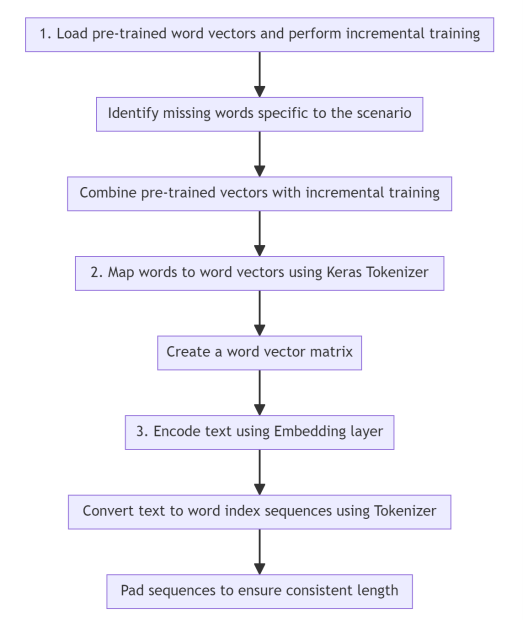
\includegraphics[width=0.6\textwidth,keepaspectratio=false]{pictures/8.png} % 修改为实际图片路径
  \caption{情感分析模块文本特征提取流程}
\end{figure}

\subsubsection{基于CNN与Bi-LSTM的混合模型构建}

结合CNN和BLSTM模型来提取和分析文本特征。
CNN 的优势是可以从全局信息中提取序列特征,并考虑这些特征之间的关系, 
而 BLSTM 不仅解决了长期依赖的问题,同时也能考虑上下文的关系。因此我们可以将两个模型结合起来使用进行探索,
用 CNN 卷积层将提取局部特征,
然后 BLSTM 层将使用特征排序来了解输入的文本排序。

\vskip 0.2cm
\noindent
\textbf{局部特征提取}

文本的局部特征主要由卷积神经网络(CNN)模型提取,CNN的核心由卷积层和池化层两部分组成。

在卷积层中,首先使用不同尺寸的卷积核对已经向量化的文本进行卷积操作。
卷积操作是指每个卷积核按照一定步长对输入的文本矩阵进行扫描,计算文本矩阵被扫描到的当前区域与卷积核之间的点积,
从而生成特征矩阵。不同尺寸的卷积核代表不同大小的感受野,使用不同尺寸的卷积核进行卷积能够提取出更加丰富的局部语义信息。
为了提高模型的表达能力,卷积操作提取的文本特征矩阵需要经过激活函数进行非线性转换。可以选择ReLU作为激活函数,
与其他激活函数相比,ReLU函数没有复杂的指数运算,收敛速度较快,并且在一定程度上能够解决梯度消失问题。

ReLU函数的计算公式为:

\begin{equation}
  \text{ReLU}(x) = \max(0, x)
\end{equation}
  
在池化层,需要对卷积层输出的特征进行进一步筛选,从而降低特征维度。本文选择最大池化对文本特征矩阵进行池化操作,即只保留特征矩阵中最突出的一个特征,舍弃其他特征。经过池化后,卷积层输出的原本维度不同的特征向量能够被转化为相同维度。

\vskip 0.2cm
\noindent
\textbf{上下文信息获取}

文本的全局特征主要由双向长短期记忆网络(Bi-LSTM)模型提取。LSTM是一种特殊的循环神经网络(RNN),
通过引入“门控机制”筛选信息,缓解了传统RNN易出现的“梯度消失”和“梯度爆炸”问题。
LSTM模型主要由三个不同的“门”和一个“记忆细胞”构成,这三个“门”分别是“忘记门”、“输入门”和“输出门”。

\begin{figure}[H]
  \centering
  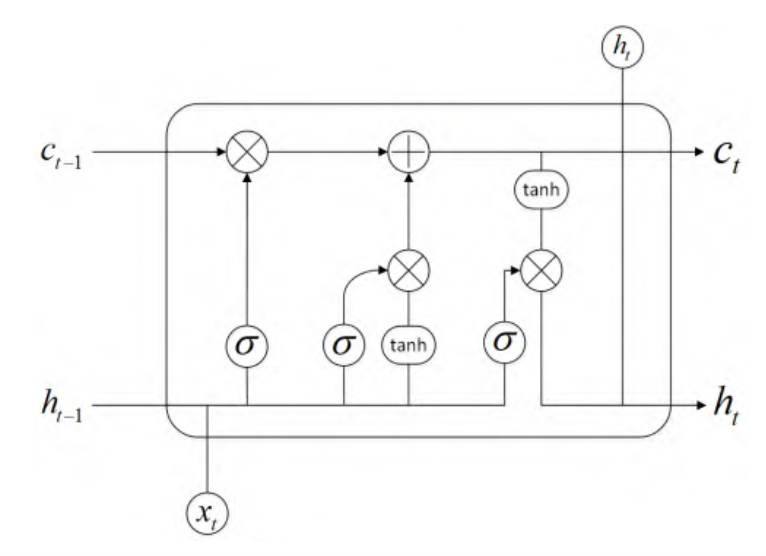
\includegraphics[width=0.5\textwidth,keepaspectratio=false]{pictures/47.png} % 修改为实际图片路径
  \caption{模型结构}
\end{figure}

“忘记门”决定哪些信息需要删除,无法继续传送下去,其公式如下:

\begin{equation}
  ft = \sigma(Wf \cdot [h{t-1}, xt] + b_f)
\end{equation}

“输入门”决定哪些信息应保留并传递给“记忆细胞”,其公式如下:

\begin{equation}
  it = \sigma(Wi \cdot [h{t-1}, xt] + b_i) 
\end{equation}

经过“输入门”的筛选后,“记忆细胞”进行更新,其公式如下:

\begin{equation}
  Ct = ft \cdot C{t-1} + it \cdot \tanh(WC \cdot [h{t-1}, xt] + bC) 
\end{equation}

“输出门”决定哪些信息应保留并输出,其公式如下:

\begin{equation}
  ot = \sigma(Wo \cdot [h{t-1}, xt] + b_o) 
\end{equation}

当前时刻的隐藏状态由输出门和记忆细胞共同决定,其公式如下:

\begin{equation}
  ht = ot \cdot \tanh(C_t) 
\end{equation}

LSTM模型通过选择性“记忆”与“更新”信息,但仅考虑了上文信息,未考虑下文信息。Bi-LSTM模型通过前向和后向的LSTM模型叠加,
实现了同时获取上下文信息。 

\begin{figure}[H]
  \centering
  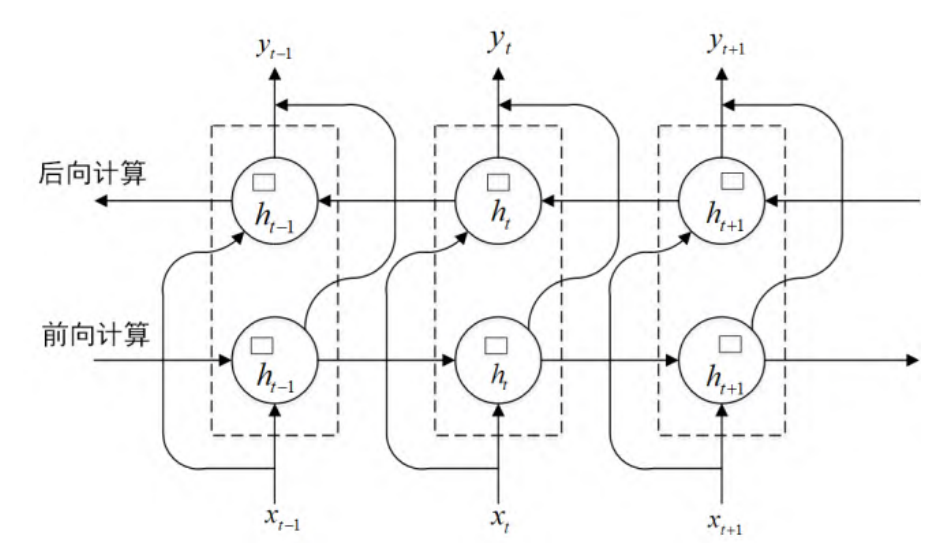
\includegraphics[width=0.7\textwidth,keepaspectratio=false]{pictures/48.png} % 修改为实际图片路径
  \caption{模型原理}
\end{figure}

Bi-LSTM模型在时刻t的隐藏状态$ ht $由前向LSTM模型的隐藏状态$h{\rightarrow t} $和后向LSTM模型的隐藏状态$ h{\leftarrow t} $拼接而成,其公式如下:

\begin{equation}
  ht = [h{\rightarrow t}, h{\leftarrow t}] 
\end{equation}

Bi-LSTM模型的最终目的是进行文本分类,因此只需要提取Bi-LSTM模型最后一个时刻的输出作为特征,这一输出包含了上下文语义信息。与CNN和LSTM模型相比,Bi-LSTM模型能够提取出更丰富的全局语义信息。

\vskip 0.2cm
\noindent
\textbf{模型结构}

结合CNN和BLSTM模型来提取和分析文本特征。CNN 的优势是可以从全局信息中提取序列特征,并考虑这些特征之间的关系, 而 BLSTM 不仅解决了长期依赖的问题,同时也能考虑上下文的关系。因此我们可以将两个模型结合起来使用进行探索,用 CNN 卷积层将提取局部特征,然后 BLSTM 层将使用特征排序来了解输入的文本排序。

\begin{figure}[H]
  \centering
  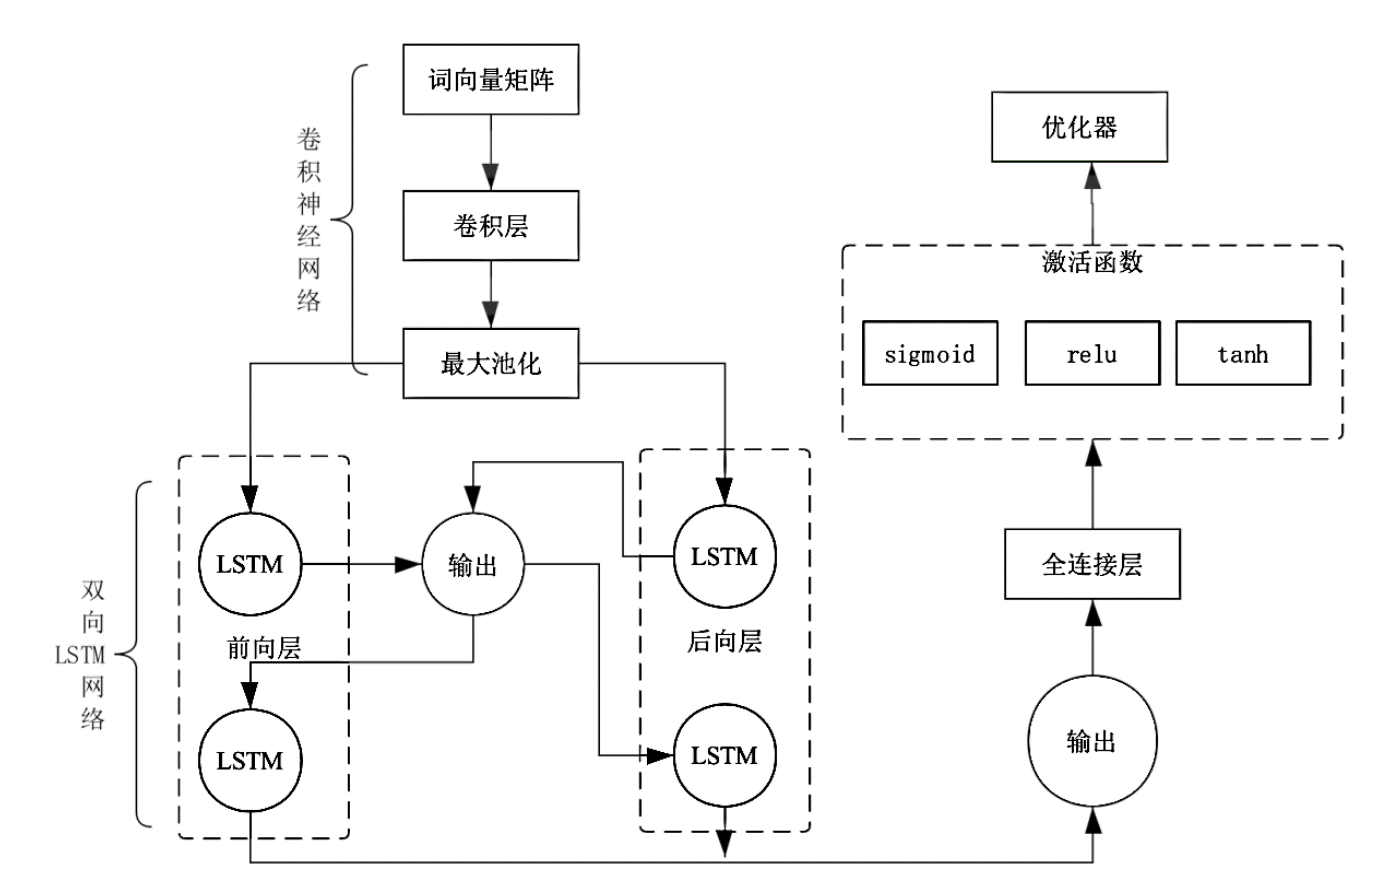
\includegraphics[width=0.7\textwidth,keepaspectratio=false]{pictures/9.png} % 修改为实际图片路径
  \caption{模型架构}
\end{figure}

\noindent
功能:通过CNN提取局部特征,通过BLSTM获取上下文信息,最终进行分类。

\noindent
步骤: 

\noindent
1 使用词向量表示文本。

与上述步骤一致。

\noindent
2使用 CNN 提取文本特征。

通过卷积和池化操作提取有效的特征。

\noindent
3使用 BLSTM 获取上下文信息。

BLSTM 使用前向 LSTM 获得输入序列历史信息,后向的 LSTM 可以获得输入序列的信息。使用特征排序来了解输入的文本排序。

\noindent
4使用分类器进行文本倾向分类。

文本倾向分类就是将全连接层的输出输入到激活函数层进行预测,如果预测结果是 Y,实际上是 Y’,则使用交叉熵作为损失函数,然后利用优化器对模型参数进行优化,同样的为了防止过度拟合,使用 dropout 机制,dropout 概率为 20%。 



实际应用中,通过CNN提取局部特征,通过BLSTM获取上下文信息,最终进行分类。

具体实施步骤:


\vskip 0.2cm
\noindent
\textbf{使用 CNN 提取文本特征}

通过卷积和池化操作提取有效的特征。CNN 由输入层、卷积层、池化层和输出层构成。第一层是输入层,使用向量矩阵作为 CNN 模型的输入,就是把语料库中的矩阵作为输入进行词嵌入;第二层是卷积层,利用卷积核从字向量矩阵提取局部特征,词向量为 96 维时,采用 3×100,4×100,5×100 大小滤波器各 250 个,padding 设置为 VALID,strides 为 1;第三层是池化层,将不用的特征进行舍弃,保留有用的特征,生成固定维度的特征向量。

\vskip 0.2cm
\noindent
\textbf{使用 BLSTM 获取上下文信息}

BLSTM 使用前向 LSTM 获得输入序列历史信息,后向的 LSTM 可以获得输入序列的信息。两个双向 LSTM 被堆叠,第一个双向 LSTM 输出返回序列作为第二个双向 LSTM 的输入,第二个双向 LSTM 输出时前向和后向最后一个单元输出的串联,最后进行叠加。BLSTM 的第一层是嵌入层,把嵌入层的矩阵作为输入,词向量维度为 96 维;第二层和第三层都是隐藏层,隐藏层大小为250。

\vskip 0.2cm
\noindent
\textbf{使用分类器进行文本倾向分类}

文本倾向分类就是将全连接层的输出输入到激活函数层进行预测,如果预测结果是 Y,实际上是 Y’,则使用交叉熵作为损失函数,然后利用优化器对模型参数进行优化,同样的为了防止过度拟合,使用 dropout 机制,dropout 概率为 20%。 

\subsubsection{模型训练和评估}

在模型构建完成后,需要对模型进行训练,并使用验证集评估模型性能。我们重点解决数据集划分、训练过程中的过拟合问题。

以下为实施步骤:

1、数据集划分:将数据集划分为训练集和验证集。

2、训练模型:使用训练集对模型进行训练。

3、评估模型:使用验证集评估模型性能,并调整参数。

\subsubsection{结果分析}

由于情感分析需要具体到个体案例分析,此处模型测试仅针对Transformer库中的预训练模型进行测试,从而论证情感分类在舆情分析中可以发挥
不容忽视作用。

本次采用github上下载开源情感分类数据集进行模型测试。

\lstinputlisting{sentiment_data.txt}

我们可以得到以下测试文本的分类结果:

\begin{table}[H]
  \centering
  \begin{tabular}{ccc}
  \toprule
  部分测试文本&分类结果&置信度\\
  \midrule
  我今天很开心,...& \cellcolor{green!20}POSITIVE & 0.9998\\
  这个产品太差劲了,...& \cellcolor{red!20}NEGATIVE & 0.9991\\
  服务态度非常好,...& \cellcolor{green!20}POSITIVE & 0.9999\\
  这部电影让我很失望,...& \cellcolor{red!20}NEGATIVE & 0.9987\\
  天气真好,适合出去玩,...& \cellcolor{green!20}POSITIVE & 0.9997\\
  我的电脑坏了,我很郁闷,...& \cellcolor{red!20}NEGATIVE & 0.9985\\
  这是我吃过最好吃的披萨。& \cellcolor{green!20}POSITIVE & 0.9998\\
  这家餐厅的服务让人无语,...& \cellcolor{red!20}NEGATIVE & 0.9978\\
  我对这次旅行非常满意,...& \cellcolor{green!20}POSITIVE & 0.9996\\
  他总是迟到,真让人生气,...& \cellcolor{red!20}NEGATIVE & 0.9990\\
  \bottomrule
  \end{tabular}
  \caption{展示的部分测试文本情感分类结果}
\end{table}

由常识判断,预训练模型的准确度极高。而后续的实例则数据集更加具有针对性、模型也依据训练数据二次训练与微调,其精确度可以保障。

我们将大数据集分为三个小数据集,作为时间序列的三个渐进时间点,对其进行ARIMA模型的应用,得到结果如下图所示:(此处展示后续预测的三个未来时间点)

\begin{figure}[H]
  \centering
  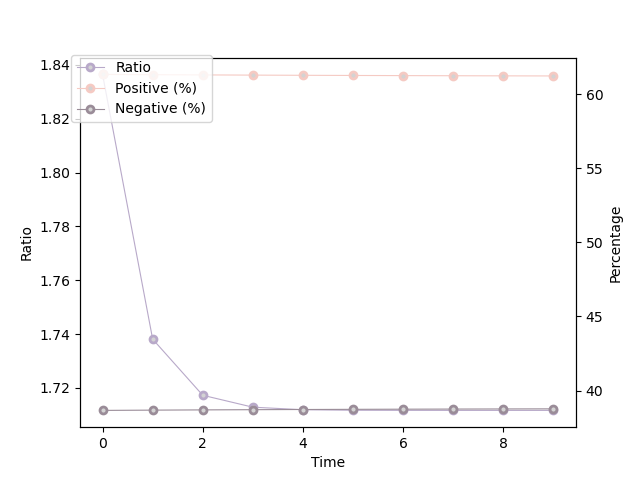
\includegraphics[width=0.6\linewidth,keepaspectratio=false]{pictures/41.png} % 修改为实际图片路径
  \caption{未来时间点的情感分类预测}
\end{figure}

\begin{figure}[H]
  \centering
  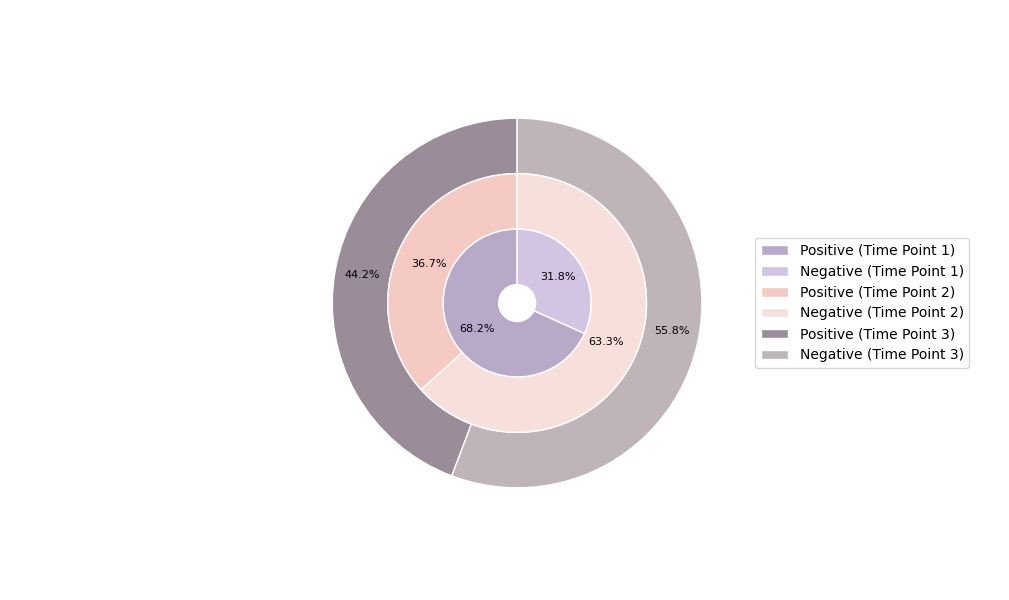
\includegraphics[width=1\linewidth,keepaspectratio=false]{pictures/42.png} % 修改为实际图片路径
  \caption{未来时间点的情感分类预测饼图}
\end{figure}

 可以看到,我们的模型在预测未来大众情感倾向上是可行有效的。

\subsection{大模型引入}

“大模型分析”模块是对其他分析模块(热点话题识别、情感分析、趋势分析)
输出的数据进行整合,生成最终的舆情分析报告。通过引入大模型(本系统使用ChatGPT大模型),
可以实现对多源数据的综合分析,提供更深层次的洞察和预测。

\begin{figure}[H]
  \centering
  
\includegraphics[width=0.2\textwidth,keepaspectratio=false]{pictures/22.png} % 修改为实际图片路径
  \caption{大模型ChatGPT}
\end{figure}


\subsubsection{数据准备与预处理}

\vskip 0.2cm
\noindent
\textbf{数据收集}

从热点话题识别、情感分析和趋势分析模块收集输出的数据。确保每个模块输出的数据准确有代表性,并且格式统一,便于后续整合。

\textbf{热点话题识别模块输出:}每条记录包含具体话题、关键词、热度评分等信息。

\textbf{情感分析模块输出:}每条记录包含文本内容、情感分类(正面、负面、中性)和情感评分。

\textbf{趋势分析模块输出:}每条记录包含文本内容、趋势指标(增长率、未来发展方向)、趋势评分等信息。

\vskip 0.2cm
\noindent
\textbf{数据整合}

使用Pandas库将不同模块的输出数据整合为一个综合数据集。包括加载模块数据,数据清洗,数据合并,
数据转换(转换成向量,便于大模型输入)等步骤。

\subsubsection{ChatGPT的Prompt设计}

\vskip 0.2cm
\noindent
\textbf{热点话题识别模块}

让 ChatGPT 进行整体热度分析,生成一个综合的热度分析报告,
包含每个话题的热度对比、总体趋势和建议。

输入数据格式:
\begin{equation}
  \text{{\{"话题": "具体话题", "关键词": ["关键词1", "关键词2", "关键词3"], "热度评分": 具体评分\}}}
\end{equation}

Prompt示例:

\begin{mdframed}[backgroundcolor=lightgray!20, linecolor=darkgray, linewidth=1pt]
  请基于以上数据进行整体热度分析,并生成一份报告。
输出格式:

1. 每个话题的综合热度分析,包括关键词和热度评分。

2. 各话题的热度对比,说明哪些话题最热门,哪些话题相对较冷。

3. 总体趋势分析,总结当前舆情的主要方向和变化趋势。

4. 提出建议,说明如何利用当前的热点话题来制定策略。
  \end{mdframed}

为了确保模型输出符合预期,可以进行如下调试。根据与预期结果的偏差,重新改进数据、提示词等,
以获得最优可读性强的模型反馈:

- 确保每个话题的热度分析准确反映关键词和评分。

- 对比各话题热度,突出最热门和最冷门的话题。

- 总体趋势应总结当前数据中的主要方向和变化趋势。

- 提出的建议应结合热度分析结果,具有可操作性。

\vskip 0.2cm
\noindent
\textbf{情感分析模块}

让 ChatGPT 进行整体情感分析,生成一个综合的情感分析报告,
包含情感分布、总体情感趋势和建议。

输入数据格式:
\begin{equation}
  \text{{\{"评论": "具体评论内容", "情感倾向": "正面/中性/负面", "情感评分": 具体评分\}}}
\end{equation}

Prompt示例:

\begin{mdframed}[backgroundcolor=lightgray!20, linecolor=darkgray, linewidth=1pt]
请基于以上数据进行整体舆情趋势分析,并生成一份综合报告。
输出格式:

1. 情感分布分析,包括正面、负面和中性情感的比例。

2. 总体情感趋势,总结当前评论的主要情感方向。

3. 提出建议,说明如何利用当前的情感分析结果来制定策略。
\end{mdframed}

	为了确保模型输出符合预期,可以进行如下调试。根据与预期结果的偏差,重新改进数据、提示词等,
  以获得最优可读性强的模型反馈:

  - 确保情感分布分析准确反映数据中的情感倾向和评分。

  - 总体情感趋势应总结当前数据中的主要情感方向。

  - 提出的建议应结合情感分析结果,具有可操作性。
  

\vskip 0.2cm
\noindent
\textbf{趋势分析模块}

让 ChatGPT 进行整体趋势分析,生成一个综合的趋势分析报告,
包含趋势分布、总体趋势和建议。

输入数据格式:
\begin{equation}
  \text{{\{"评论": "具体评论", "趋势预测": "具体趋势预测", "未来发展方向":"具体未来发展方向","趋势评分": 8\}}}
\end{equation}

Prompt示例:

\begin{mdframed}[backgroundcolor=lightgray!20, linecolor=darkgray, linewidth=1pt]
请基于以上数据进行整体舆情趋势分析,并生成一份综合报告。
输出格式:

1. 趋势分布分析,包括各趋势的比例。

2. 总体趋势,总结当前评论的主要趋势方向。

3. 提出建议,说明如何利用当前的趋势分析结果来制定策略。
\end{mdframed}

为了确保模型输出符合预期,可以进行如下调试。根据与预期结果的偏差,重新改进数据、提示词等,
以获得最优可读性强的模型反馈:

- 确保趋势分布分析准确反映数据中的趋势预测和评分。

- 总体趋势应总结当前数据中的主要趋势方向。

- 提出的建议应结合趋势分析结果,具有可操作性。

\vskip 0.2cm
\noindent
\textbf{综合分析}

为了能使大模型更好的切合公司现状以及发展方向,可以补充背景信息、发展方向等其他Prompt,如:

\begin{mdframed}[backgroundcolor=lightgray!20, linecolor=darkgray, linewidth=1pt]
背景信息:

1. 公司在最近一个季度发布了一款新产品,市场反响热烈,获得了很多好评。

2. 最新市场调查显示,消费者对公司的服务满意度有所下降,需要关注服务质量。

3. 许多公司在科技创新方面投入了大量资源,本季度的热门话题是科技研发和创新。

\end{mdframed}

\begin{mdframed}[backgroundcolor=lightgray!20, linecolor=darkgray, linewidth=1pt]
发展方向:

1. 增强客户服务和客户满意度,以应对服务质量下降的问题。

2. 持续投入科技研发,推动创新,以保持市场竞争力。

3. 关注市场反响和用户反馈,优化新产品性能和用户体验。


\end{mdframed}


\section{展示层}

\subsection{综合分析生成报告文本}

生成自然语言报告需要从模型推理结果中提取关键信息,
并将这些信息整合成易于理解的自然语言形式。根据前文给定输出数据结果、提示词设计,利用大模型
生成可读性强的分析报告。

\subsubsection{情感分析部分}

使用大模型对数据进行综合分析阐述,对于结果加以概括。情感分析部分需要描述整体情感分布,例如:“在分析的文本中,正面情感占比为X%,负面情感占比为Y%,中性情感占比为Z%。整体来看,xx情感站主导,可见大部分客户对于本产品持xx态度。”同时给出相应具体实例,说明各类情感的典型文本。

\subsubsection{热点话题部分}

使用热点话题识别结果,描述每个热点话题的关键词和热度。列出识别出的热点话题及其热度,例如:“本次分析共识别出5个热点话题,分别为A、B、C、D和E,其中话题A的热度最高。”同时提供每个话题的关键词和相关示例。

\subsubsection{趋势分析部分}
对大模型不断投喂与训练,针对现有数据尝试预测未来舆情变化与发展。对于所得结果描述舆情变化的趋势,例如:“在过去一个月中,关于公司的正面情感呈上升趋势,负面情感有所下降。”描述预测未来的发展方向,例如:“预计未来两周内,正面情感将继续上升,负面情感将保持稳定。”

\subsubsection{综合分析与结论部分}

总结各部分的分析结果,提出整体的舆情结论。对于以上结果,进行综合分析,例如:“综合以上分析结果,可以得出结论,公司在近期的公众舆情中表现良好,正面情感占多数。”同时提出建议或行动方案,例如:“建议公司继续保持良好的市场表现,针对负面情感较集中的话题进行重点关注和处理。”

最终将上述部分整合,确保上述部分有有效逻辑连接,整体连贯一致。之后选择合适的格式进行输出。

\definecolor{morandiLight}{RGB}{207, 184, 169}
\definecolor{morandiDark}{RGB}{105, 89, 80}
\begin{mdframed}[backgroundcolor=morandiLight!30, linecolor=morandiDark, linewidth=1pt]


\begin{center}
  秦Plus和宋Plus综合报告示例
\end{center}

1. 情感分析

- 正面情感(65%):用户对设计、性能和油耗经济性满意。

- 负面情感(20%):主要集中在车内噪音、悬挂硬度和售后服务。

- 中性情感(15%):日常驾驶体验和内饰设计。

结论:整体情感正面,设计和经济性受好评。


2. 热点话题

- 设计与外观(热度评分:8.5):时尚设计受欢迎。

- 油耗与经济性(热度评分:8.0):油耗表现优秀。

- 驾驶体验(热度评分:7.8):操控和舒适性好。

- 车内噪音(热度评分:6.5):部分用户抱怨噪音大。

- 售后服务(热度评分:5.5):服务态度和效率有待提高。

结论:设计和油耗表现突出,噪音和售后需改进。


3. 趋势分析

- 近期趋势:正面情感上升,负面情感下降。

- 未来预测:正面情感将继续上升,负面情感稳定。

结论:受欢迎度有望提升,需关注用户反馈改进。


4. 综合结论与建议

综合结论:秦Plus和宋Plus总体表现良好,用户满意度高。需改进车内噪音和售后服务。

建议:

- 保持优势:强化设计和经济性宣传。

- 改进不足:解决噪音问题,优化售后服务。

- 用户互动:通过社交媒体与用户互动,及时解决问题。

\end{mdframed}


\subsection{结论可视化展示}

针对分析层各模块所得数据进行可视化展示,辅助对于舆情分析的综合判断。
其中工具所需工具有:

1. Matplotlib:功能强大,适合绘制各种类型的图表。适用于趋势分析曲线图、词频分布直方图等。

2.Seaborn:基于Matplotlib,提供更加美观和高级的绘图接口。适用于热力图、分布图、回归图等。

3.Plotly:交互性强,适合制作动态和交互式图表。适用于交互式趋势图、词云等。

4. D3.js:高度可定制化,适合生成复杂的动态和交互式图表。适用于需要高度定制化和交互性的图表。


以下依次介绍报告中各板块展示方法:


\subsubsection{舆情分析曲线图}

从分析层获取舆情趋势分析的数据,包括时间和对应的情感指数。
并对数据进行清洗和整理,确保时间序列数据完整且有序。使用Matplotlib绘制舆情趋势分析曲线图

通过图像绘制,能够直观具体的看出舆情走势以及未来发展趋向,如下图所示:

\begin{figure}[H]
  \centering
  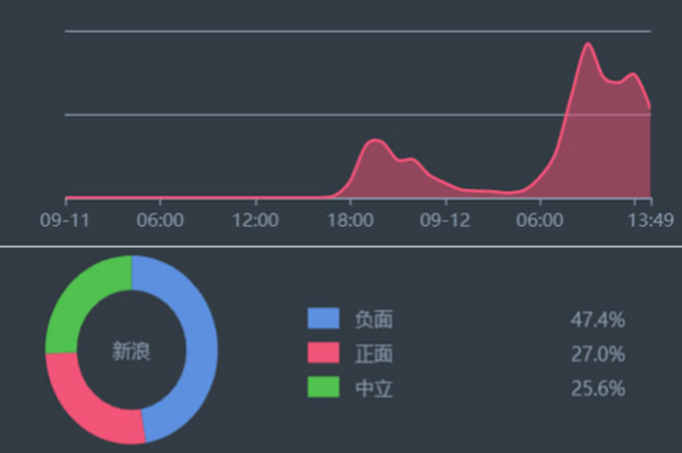
\includegraphics[width=0.6\textwidth,keepaspectratio=false]{pictures/4.png} % 修改为实际图片路径
  \caption{热点趋势分析曲线图示例}
\end{figure}

\subsubsection{热点词云图}

从热点话题识别模块获取关键词及其频数并对关键词进行计数,整理成频数数据。使用Plotly绘制热点词云图。

其能够明确了解公众对于产品的评价,辅助公司对于产品的公众定位,如下图所示:

\begin{figure}[H]
  \centering
  
\includegraphics[width=0.6\textwidth,keepaspectratio=false]{pictures/5.png} % 修改为实际图片路径
  \caption{热点词云图示例}
\end{figure}



\subsubsection{情感分析饼图}

从情感分析模块获取各情感类型的比例数据,整理成比例形式使用Matplotlib绘制情感分布饼图。

通过饼图绘制,能够直接了然地看出公众对于产品的情感态度,辅助公司对产品的进一步调整。

\begin{figure}[H]
  \centering
  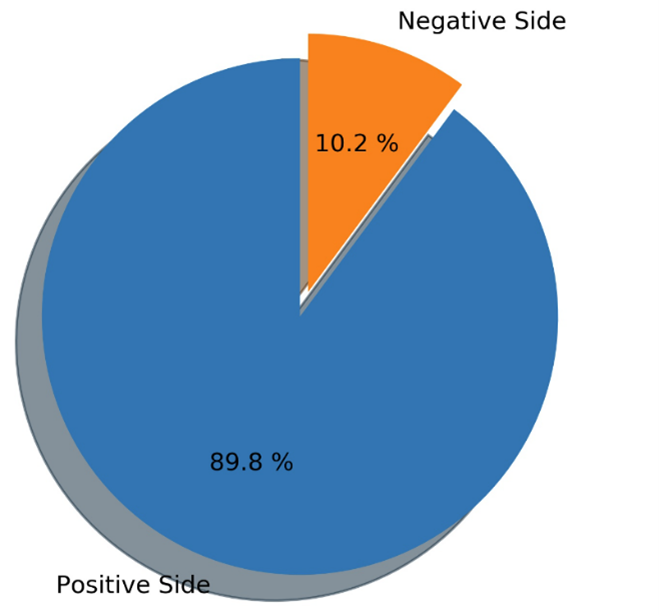
\includegraphics[width=0.3\textwidth,keepaspectratio=false]{pictures/35.png} % 修改为实际图片路径
  \caption{饼图示意}
\end{figure}

\subsubsection{热力图}

从分析层获取热点话题与情感分布的交叉数据。将数据整理成矩阵形式,以便绘制热力图并使用Seaborn绘制热力图。

应用上述方法,可整体高效地看出公众对于产品的态度并通过关键字分析出客户需求,利于公司对产品的进一步优化。

\begin{figure}[H]
  \centering
  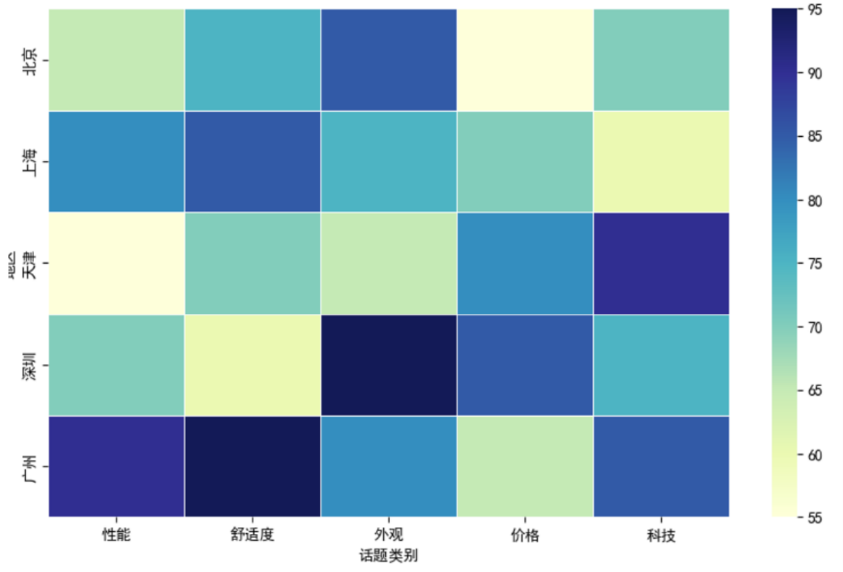
\includegraphics[width=0.5\textwidth,keepaspectratio=false]{pictures/6.png} % 修改为实际图片路径
  \caption{热力图示意}
\end{figure}


通过上述板块数据可视化,我们得到了完整的可视化报告,可供用户直观的获取当今舆情的相关信息。

\section{实例应用}

\subsection{实例简介}

该智能舆情分析系统实例专注于汽车品牌管理,通过爬虫技术从百度有驾网站采集汽车评论数据,
并对数据进行综合处理和分析。系统利用分词和TF-IDF算法从评论中提取关键词,
并通过热度图和词云展示关键词的频率。通过text-CNN模型进行情感分析,系统能够评估各维度的消费者情绪,
并通过时间序列分析监测市场趋势。
整个实例为汽车品牌提供了全面的市场分析和管理策略支持。

\begin{figure}[H]
  \centering
  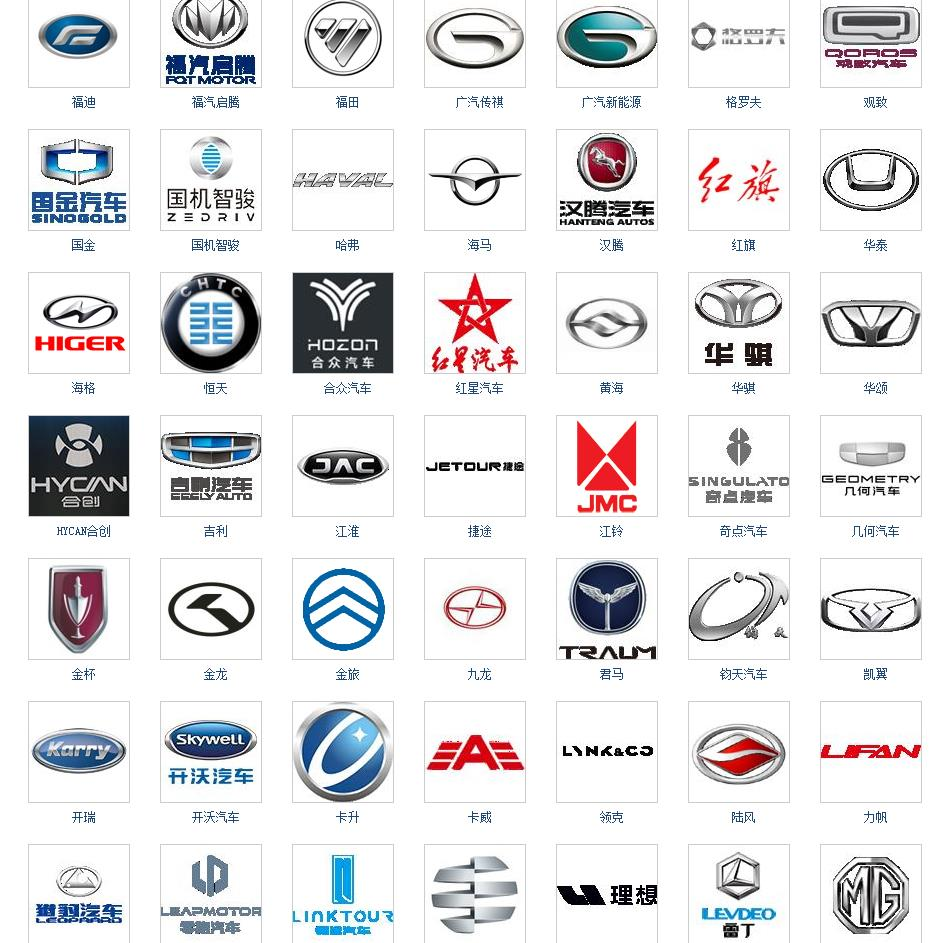
\includegraphics[width=0.6\textwidth,keepaspectratio=false]{pictures/34.png} % 修改为实际图片路径
  \caption{汽车品牌管理}
\end{figure}

\subsection{数据收集与预处理}

\subsubsection{数据采集}

导入库:

\begin{mdframed}[backgroundcolor=darkgray, linecolor=lightgray, linewidth=1pt, innermargin=0.5cm, outermargin=0.5cm, skipbelow=0.1cm]
  \color{white}
  \begin{verbatim}
  import requests
  import json
  import time
  import re    
  \end{verbatim}
  \vspace{-1.5em} % 调整文本和底部边缘的距离
  \end{mdframed}

  导入代码所需要的python库,其中requests库是请求库,用于发送HTTP请求,json库用于处理json数据,time库用于控制请求之间的延迟。

  常量定义:

  \begin{mdframed}[backgroundcolor=darkgray, linecolor=lightgray, linewidth=1pt, innermargin=0.5cm, outermargin=0.5cm, skipbelow=0.1cm]
    \color{white}
    \begin{verbatim}
  MOBILE_TOKEN = '1_2298dc2ac944caad6d611cdbbcb9710e'
  DESKTOP_TOKEN = '1_526c1239fc0b0512a2bd13ac6b962f5f'
  DATA_PRODUCER = 2
  DELAY = 0.1  # 请求之间的延迟,单位为秒
  DESKTOP_TAGS = [
      'all', 'space', 'fuel', 'cruising', 'workmanship,internal,external',
      'powersteering,power,control', 'comfort', 'cp', 'select'
  ]
  MOBILE_TAGS = [
      'all', 'space', 'consumption', 'cruising', 'workmanship',
      'powersteering', 'select_process', 'cp'
  ]
  SERIES_IDS = ['1005964']
  
  HEADERS = {
      'User-Agent': 'Mozilla/5.0 (Windows NT 10.0; Win64; x64) AppleWebKit/537.36 ...
      'Accept': 'application/json, text/javascript, */*; q=0.01',
      'Accept-Language': 'en-US,en;q=0.9',
      'Connection': 'keep-alive',
      'Referer': 'https://www.yoojia.com',
  }   
    \end{verbatim}
    \vspace{-1.5em} % 调整文本和底部边缘的距离
    \end{mdframed}

    MOBILE\_TOKEN与DESKTOP\_TOKEN用于身份验证,以便从有驾网站的API接口获取数据。DATA\_PRODUCER是数据来源标识,用于标识数据来源的类型,区分数据的不同的生产者。此处设为2确保API请求的是用户评论而非其他数据。DELAY用于控制请求之间的延迟,提高请求的成功率,避免频繁请求对服务器造成压力,导致触发反爬虫机制。DESKTOP\_TAGS与MOBILE\_TAGS是标签,用于分类不同类型的评论。SERIES\_ID用于获取特定汽车系列的ID,用于获取秦PLUS与宋PLUS的数据。HEADERS 是一个包含HTTP请求头信息的字典,用于模拟浏览器访问API接口,让爬虫伪装成正常的浏览器访问,从而绕过一些简单的反爬虫机制。


    函数定义:

    \begin{mdframed}[backgroundcolor=darkgray, linecolor=lightgray, linewidth=1pt, innermargin=0.5cm, outermargin=0.5cm, skipbelow=0.1cm]
      \color{white}
      \begin{verbatim}
  def fetch_comments(page_number, series_id, tag, sort=0, max_retries=5, delay=1):
  url = f'https://www.yoojia.com/gateway/koubei-api/koubeis/format?token={DESKTOP_TOKEN}&pn={page_number}...
  for attempt in range(max_retries):
      try:
          response = requests.get(url, headers=HEADERS)
          response.raise_for_status()  # 检查HTTP请求是否成功
          return response.json()
      except requests.exceptions.RequestException as e:
          print(f"Error fetching page {page_number}, series_id {series_id}, tag {tag} on attempt {attempt + 1}...
          time.sleep(delay)
  print(f"Failed to fetch page {page_number}, series_id {series_id}, tag {tag} after {max_retries} attempts.")
  return None
      \end{verbatim}
      \vspace{-1.5em} % 调整文本和底部边缘的距离
      \end{mdframed}

      该函数用于获取特定页面的评论数据,构建请求URL,包含页码、系列ID、标签和排序参数。尝试最多 max\_retries 次获取数据,如果成功则将HTTP响应的内容解析为JSON格式的数据并返回,否则打印错误并等待 delay 秒后重试。

  \begin{mdframed}[backgroundcolor=darkgray, linecolor=lightgray, linewidth=1pt, innermargin=0.5cm, outermargin=0.5cm, skipbelow=0.1cm]
    \color{white}
    \begin{verbatim}
  def parse_comments(data):
  comments = data.get('data', {}).get('koubei_list', [])
  parsed_comments = []
  for comment in comments:
      parsed_comments.append({
          'id': comment.get('id'),
          'car_price': comment.get('car_purchase_price'),
          'car_buytime': comment.get('purchase_time'),
          'car_buylocation': comment.get('car_purchase_location'),
          'car_name': comment.get('car_info', {}).get('car_model_name'),
          'comment': extract_comment_content(comment.get('content', []))
      })
  return parsed_comments
  \end{verbatim}
  \vspace{-1.5em} % 调整文本和底部边缘的距离
  \end{mdframed}

  该函数用于解析评论数据,将其转换为所需的格式,提取评论的ID、购车价格、购车地点、购车时间、车型以及评论内容。

  \begin{mdframed}[backgroundcolor=darkgray, linecolor=lightgray, linewidth=1pt, innermargin=0.5cm, outermargin=0.5cm, skipbelow=0.1cm]
    \color{white}
    \begin{verbatim}
  def extract_comment_content(content):
  full_text = []
  for item in content:
      full_text.append(item.get('text', ''))
  return ' '.join(full_text)  
  \end{verbatim}
  \vspace{-1.5em} % 调整文本和底部边缘的距离
  \end{mdframed}

主函数:

\begin{mdframed}[backgroundcolor=darkgray, linecolor=lightgray, linewidth=1pt, innermargin=0.5cm, outermargin=0.5cm, skipbelow=0.1cm]
  \color{white}
  \begin{verbatim}
  def main(series_ids, tags):
  for series_id in series_ids:
      all_comments = []
      for tag in tags:
          sort_range = range(2) if tag == 'all' else range(1)
          for sort in sort_range:
              page_number = 1
              while True:
                  print(f'Fetching page {page_number}/76 for series_id {series_id}...
                  data = fetch_comments(page_number, series_id, tag,sort=sort)
                  if data is None:
                      break
                  comments = parse_comments(data)
                  if not comments:
                      print(f'No more comments found for series_id {series_id}...
                      break
                  all_comments.extend(comments)
                  page_number += 1

                  # 判断是否还有更多评论
                  if data.get('data', {}).get('koubei_list') == []:
                      print(f'No more comments available for series_id...
                      break
                  time.sleep(DELAY)  # 添加延迟
      file_name = f'desktop_comments_{series_id}.json'
      with open(file_name, 'w', encoding='utf-8') as f:
          json.dump(all_comments, f, ensure_ascii=False, indent=4)
      print(f'Comments for series_id {series_id} saved to {file_name}.')
\end{verbatim}
\vspace{-1.5em} % 调整文本和底部边缘的距离
\end{mdframed}

该函数用于遍历所有系列的ID和标签,同时输出是否成功获取到了评论,并将成功获取到的评论数据解析,保存到当地的json文件中。

主程序:

\begin{mdframed}[backgroundcolor=darkgray, linecolor=lightgray, linewidth=1pt, innermargin=0.5cm, outermargin=0.5cm, skipbelow=0.1cm]
  \color{white}
  \begin{verbatim}
  if __name__ == "__main__":
  series_ids = SERIES_IDS
  tags=DESKTOP_TAGS
  main(series_ids,tags)
\end{verbatim}
\vspace{-1.5em} % 调整文本和底部边缘的距离
\end{mdframed}

初始化参数:

\begin{mdframed}[backgroundcolor=darkgray, linecolor=lightgray, linewidth=1pt, innermargin=0.5cm, outermargin=0.5cm, skipbelow=0.1cm]
  \color{white}
  \begin{verbatim}
  import json
  import hashlib
  import os
  
  def hash_comment(comment):
      """
      对评论内容进行哈希处理
      """
      return hashlib.md5(comment.encode('utf-8')).hexdigest()
  
  def remove_duplicates(input_file, output_file, backup_folder):
      """
      从输入文件中读取评论,去重后保存到输出文件
      """
      with open(input_file, 'r', encoding='utf-8') as infile:
          comments = json.load(infile)
  
      unique_comments = []
      seen_hashes = {}
      duplicate_count = 0
      diff_id_count = 0
        ...
      total_comments = len(comments)
      unique_comments_count = len(unique_comments)
      backup_files_count = len(os.listdir(backup_folder))
      ...#输出提示
  if __name__ == "__main__":
      input_files = ['desktop_comments_1005761.json',...
      output_files = ['desktop_宋PLUS新能源.json', 'desktop_秦PLUS.json']
      backup_folder = 'backup_duplicates'
  
      for input_file, output_file in zip(input_files, output_files):
          remove_duplicates(input_file, output_file, backup_folder)
\end{verbatim}
\vspace{-1.5em} % 调整文本和底部边缘的距离
\end{mdframed}

同时,我们考虑到可能会有重复的数据出现,所以我们需要以上代码来处理和去重数据。以上代码从输入文件中读取评论数据,利用哈希函数对评论内容进行哈希处理,从而检测重复评论。对于重复评论,程序会根据哈希值进行比较,如果发现不同ID的重复评论,则将这些评论备份到指定的备份文件夹中。同时,程序会记录总评论数、唯一评论数、重复评论数以及不同ID但内容重复的评论数,并将去重后的评论保存到输出文件中。

首先,定义函数,接受评论内容并返回其MD5哈希值,用于唯一标识评论内容。接着主函数读取输入文件中的评论数据,并初始化一个空列表用于存储唯一评论,以及一个字典用于跟踪已经遇到过的评论的哈希值。然后遍历所有评论,获取哈希值并检测其是否在字典中。如果相同则根据ID判断是否相同。如果哈希值不存在于字典中,则将该评论视为唯一评论并添加到唯一评论列表中,同时将哈希值及其对应的评论ID记录到字典中。

数据去重代码:

\begin{mdframed}[backgroundcolor=darkgray, linecolor=lightgray, linewidth=1pt, innermargin=0.5cm, outermargin=0.5cm, skipbelow=0.1cm]
  \color{white}
  \begin{verbatim}
  import hashlib

  def hash_comment(comment):
      return hashlib.md5(comment.encode('utf-8')).hexdigest()
  
  def remove_duplicates(input_file, output_file, backup_folder):
      ...
      for comment in comments:
          comment_text = comment['comment']
          comment_hash = hash_comment(comment_text)
  
          if comment_hash in seen_hashes:
              # 处理重复评论
              ...
    \end{verbatim}
\vspace{-1.5em} % 调整文本和底部边缘的距离
\end{mdframed}


爬取的数据格式如图所示:

\begin{figure}[htbp]
  \centering
  
  \begin{subfigure}{0.32\textwidth}
    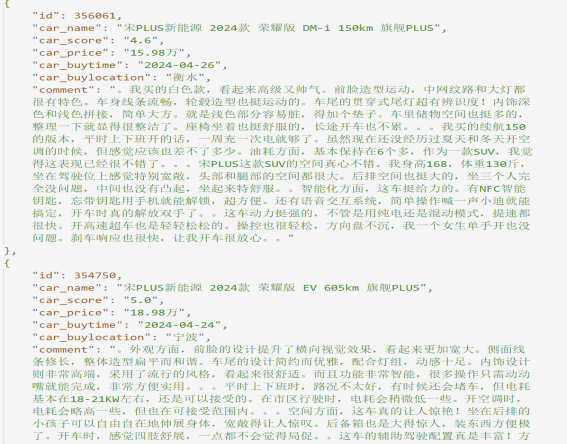
\includegraphics[width=\linewidth]{pictures/49.png}
    \caption{比亚迪秦PLUS}
  \end{subfigure}
   % 添加空白以分隔子图
  \begin{subfigure}{0.32\textwidth}
    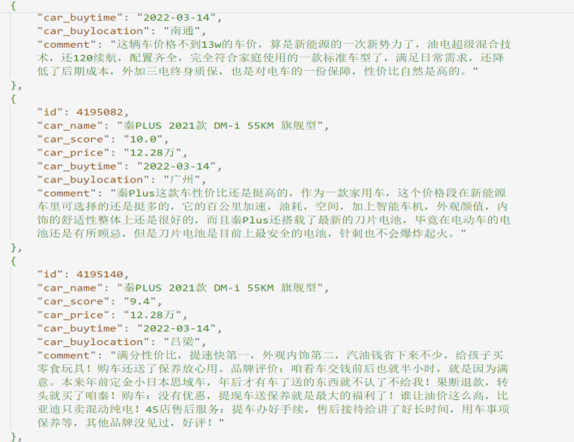
\includegraphics[width=\linewidth]{pictures/50.png}
    \caption{比亚迪宋PLUS}
  \end{subfigure}

  \end{figure}

  上述两张图是通过修改SERIES\_ID获取到的比亚迪秦PLUS和宋PLUS两款车型的示例,可以看到,爬虫成功的将用户评论的相关数据存储到了本地的json文件中

  收集数据信息如下:

  \begin{table}[H]
    \centering
    \begin{tabular}{lcc}
    \toprule
    信息 & 宋PLUS新能源 & 秦PLUS \\
    \midrule
    总评论数 & 5195 & 5848 \\
    唯一评论数 & 2584 & 2602 \\
    重复评论数 & 2611 & 3246 \\
    重复但ID不同的评论数 & 27 & 30 \\
    备份文件数 & 7 & 14 \\
    \bottomrule
    \end{tabular}
    \caption{数据去重结果}
\end{table}

去重完成后,去重后的评论分别保存到 \texttt{output/desktop\_宋PLUS新能源.json} 和 \texttt{output/desktop\_秦PLUS.json}。通过去重处理,确保数据的唯一性和准确性,提高了分析结果的可靠性。

\subsubsection{评论角度分类}

在本实例中,我们对汽车评论进行角度分类,以便分析用户对不同方面的评价。分类过程如下:

\noindent 
1.	加载与保存JSON文件:

使用\texttt{load\_json}函数加载包含评论的JSON文件,使用\texttt{save\_json}函数保存分类结果,确保目录存在。

\noindent 
2.	切分评论:

评论切分是基于特定的分隔符,例如句号、感叹号、换行符等。切分函数\texttt{split\_comment}依据不同的特征进行句子分割,返回分割后的句子列表和分割方法的标识符。

示例代码(省略部分细节):

\begin{mdframed}[backgroundcolor=darkgray, linecolor=lightgray, linewidth=1pt, innermargin=0.5cm, outermargin=0.5cm, skipbelow=0.1cm]
  \color{white}
  \begin{verbatim}
  def split_comment(comment_text):
    sentences = None
    if len(re.findall(r'[。 !] ', comment_text)) >= 3:
        sentences = re.split(r'[。 !] ', comment_text)
        split_id = 1
    elif len(re.findall(r'\n【', comment_text)) >= 2:
        sentences = re.split(r'\n【|\】', comment_text)
        split_id = 2
  # 其他切分方案省略

	elif len(re.findall(r'(。|\.\.\.|\\n)|((?<![0-9a-zA-Z]) (?![0-9a-zA-Z]))|;|;',...
		sentences = re.split(r'(。|\.\.\.|\\n)|((?<![0-9a-zA-Z]) (?![0-9a-zA-Z]))|;|;',...
		split_id = 6
    else:
        return -1, [comment_text]
    sentences = [sen.strip() for sen in sentences if sen and sen.strip() ...
    return split_id, sentences
    \end{verbatim}
\vspace{-1.5em} % 调整文本和底部边缘的距离
\end{mdframed}

3.	提取分类:

根据预定义的关键词表,将句子分类到不同的评价角度,如外观与内饰、操控与性能、舒适性等。提取分类的函数extract\_aspects会扫描句子中是否包含任何与某个角度相关的关键词。

示例代码(省略部分细节):

\begin{mdframed}[backgroundcolor=darkgray, linecolor=lightgray, linewidth=1pt, innermargin=0.5cm, outermargin=0.5cm, skipbelow=0.1cm]
  \color{white}
  \begin{verbatim}
  def extract_aspects(sentence):
    aspect_keywords = {
      "操控与性能": ["刹车", "加速", "驾驶", "制动", "超车",...
      "舒适性": ["舒适", "悬挂", "减震", "隔音", "安静",...
		  # 其他分类和关键词省略
    }
    aspects = []
    for aspect, keywords in aspect_keywords.items():
        if any(keyword in sentence for keyword in keywords):
            aspects.append(aspect)
    return aspects
    \end{verbatim}
\vspace{-1.5em} % 调整文本和底部边缘的距离
\end{mdframed}

4.	分类评论:

使用classify\_comments函数对每条评论进行切分和分类。对切分后的每个句子,根据其包含的关键词确定其分类角度。

对于无法切分或未能分类的评论,分别记录下来以便进一步分析。

核心代码(省略部分细节):

\begin{mdframed}[backgroundcolor=darkgray, linecolor=lightgray, linewidth=1pt, innermargin=0.5cm, outermargin=0.5cm, skipbelow=0.1cm]
  \color{white}
  \begin{verbatim}
  def classify_comments(comments):
  classified_comments = []
  no_split_comments = []
  # ... other definitions

  for comment in comments:
      comment_text = comment['comment']
      split_id, sentences = split_comment(comment_text)
      if split_id != -1:
          for index, sentence in enumerate(sentences):
              aspects = extract_aspects(sentence)
              sen_id = f"{comment['id']}_{index}"
              unique_comments.append({
                  'sen_id': sen_id,
                  'car_name': comment['car_name'],
                  'sentence': sentence,
                  'aspects': ', '.join(aspects),
                  'split_id': split_id
              })
              if aspects:
                  for aspect in aspects:
                      classified_comment = {
                          'aspect': aspect,
                          'sen_id': sen_id,
                          # ... other similiar fields
                      }
                      classified_comments.append(classified_comment)
                      aspect_count[aspect] = aspect_count.get(aspect, 0) + 1
              else:
                  no_aspect_comments.append({
                      # ... similar fields
                  })
      else:
          no_split_comments.append({
              'id': comment['id'],
              'car_name': comment['car_name'],
              'comment': comment_text
          })
    \end{verbatim}
\vspace{-1.5em} % 调整文本和底部边缘的距离
\end{mdframed}

分类结果:

\begin{table}[H]
  \centering
  \begin{tabular}{lcc}
      \toprule
      分类                   & 秦PLUS             & 宋PLUS 新能源     \\
      \midrule
      总评论数              & 2602               & 2584               \\
      总分条评论数          & 18649              & 17274              \\
      未成功切分的评论数    & 1                  & 0                  \\
      找不到分类的条评论数  & 606 (3.25\%)       & 745 (4.31\%)       \\
      总分类评论数          & 36572              & 34379              \\
      操控与性能            & 6891               & 6474               \\
      舒适性                & 6217               & 6080               \\
      外观与内饰            & 7235               & 7355               \\
      能耗与续航            & 3728               & 3011               \\
      空间                  & 3816               & 3877               \\
      车机硬件与智能化      & 4087               & 3848               \\
      安全                  & 689                & 734                \\
      性价比                & 3167               & 2273               \\
      品牌与服务            & 521                & 532                \\
      维保                  & 221                & 195                \\
      \bottomrule
  \end{tabular}
  \caption{分类统计结果}
\end{table}

示例输出展示(json文件):


\begin{mdframed}[backgroundcolor=lightgray!20, linecolor=darkgray, linewidth=1pt]
  \begin{verbatim}
  [
    {
        "sen_id": "356507_2",
        "car_name": "2024款 荣耀版 DM-i 150km 旗舰PLUS",
        "sentence": "这车的配置简直太智能了...
        "aspects": "车机硬件与智能化",
        "split_id": 1
    },
    {
        "sen_id": "356507_3",
        "car_name": "2024款 荣耀版 DM-i 150km 旗舰PLUS",
        "sentence": "驾驶这辆车真的挺爽的...
        "aspects": "操控与性能, 舒适性",
        "split_id": 1
    },
    {
        "sen_id": "354689_0",
        "car_name": "2024款 荣耀版 DM-i 150km 旗舰PLUS",
        "sentence": "这车的外观真的挺霸气的...
        "aspects": "外观与内饰, 性价比",
        "split_id": 1
    },
    {
        "sen_id": "354689_1",
        "car_name": "2024款 荣耀版 DM-i 150km 旗舰PLUS",
        "sentence": "宋PLUS新能源的空间真的给我留下了深刻印象...
        "aspects": "空间, 舒适性",
        "split_id": 1
    }
  ]
\end{verbatim}
  \end{mdframed}

  \begin{mdframed}[backgroundcolor=lightgray!20, linecolor=darkgray, linewidth=1pt]
    \begin{verbatim}
  [
    {
        "sen_id": "356507_2",
        "car_name": "2024款 荣耀版 DM-i 150km 旗舰PLUS",
        "sentence": "这车的配置简直太智能了,每次用都觉得像在跟未来对话一样。...
        "aspects": "车机硬件与智能化",
        "split_id": 1
    },
    {
        "sen_id": "356507_3",
        "car_name": "2024款 荣耀版 DM-i 150km 旗舰PLUS",
        "sentence": "驾驶这辆车真的挺爽的,转向手感很好,油门响应也特别快,...
        "aspects": "操控与性能, 舒适性",
        "split_id": 1
    },
    {
        "sen_id": "354689_0",
        "car_name": "2024款 荣耀版 DM-i 150km 旗舰PLUS",
        "sentence": "这车的外观真的挺霸气的,大灯设计犀利,进气格栅也显得很大气...
        "aspects": "外观与内饰, 性价比",
        "split_id": 1
    },
    {
        "sen_id": "354689_1",
        "car_name": "2024款 荣耀版 DM-i 150km 旗舰PLUS",
        "sentence": "宋PLUS新能源的空间真的给我留下了深刻印象。我身高172cm,...
        "aspects": "空间, 舒适性",
        "split_id": 1
    }
]
  \end{verbatim}
    \end{mdframed}

通过上述过程,我们实现了对汽车评论的细化分类,为后续的热词分析和情感分析提供了基础。
经验证,未成功分类的条评论几乎全部为无效信息,如开场白、小标题、简单经历分享等等,可以忽略。样例:

\begin{mdframed}[backgroundcolor=lightgray!20, linecolor=darkgray, linewidth=1pt]
  \begin{verbatim}
  {
      "id": "294028_0",
      "car_name": "2023款 冠军版 DM-i 110KM 旗舰PLUS",
      "comment": "🚗2023比亚迪宋DM-i,开启我的出行新篇章!🚗",
      "split_id": 3
  },
  {
      "id": "294028_1",
      "car_name": "2023款 冠军版 DM-i 110KM 旗舰PLUS",
      "comment": "Hey小伙伴们!今天我要给大家分享一下我的新宠,...
      "split_id": 3
  },
  {
      "id": "302141_0",
      "car_name": "2021款 EV 旗舰型",
      "comment": "【攒够买车的首付,买了宋PLUS,享受幸福时光😍😍",
      "split_id": 2
  },
  {
      "id": "301684_0",
      "car_name": "2021款 DM-i 51KM 尊荣型",
      "comment": "一直以来家人外出都需要乘坐公交车或者是打车,...
      "split_id": 3
  }
\end{verbatim}
  \end{mdframed}



\subsection{热点分析}

在本实例中,我们使用文本处理和数据可视化技术对汽车评论进行热点分析。此分析通过提取评论中的高频关键词并生成词云图来直观展示用户对不同方面的关注点。以下是实现过程的详细步骤:

\subsubsection{生成 n-gram 关键词}

1. 我们首先使用 jieba 库对评论文本进行分词,并通过自定义停用词和严格停用词进行过滤。

2. 使用 generate\_ngrams 函数生成 n-gram 关键词,并根据这些关键词计算每个词组的出现频率。

3. 停用词分为两种:严格停用词(strict\_stop),用于过滤掉无关紧要的词语;整体停用词(stopwords),用于去除无意义的高频词。

\begin{mdframed}[backgroundcolor=darkgray, linecolor=lightgray, linewidth=1pt, innermargin=0.5cm, outermargin=0.5cm, skipbelow=0.1cm]
  \color{white}
  \begin{verbatim}
  def generate_ngrams(text, n, stopwords, strict_stop):
  words = jieba.lcut(text)
  words = [word.upper() for word in words]
  words = [word for word in words if word not in stopwords]
  ngrams = zip(*[words[i:] for i in range(n)])
  ngrams = [ngram for ngram in ngrams if not any(ssword in word for ssword in strict_stop...
  ngrams = [''.join(ngram) for ngram in ngrams]
  ngrams = [ngram for ngram in ngrams if ngram not in stopwords]
  return ngrams
\end{verbatim}  
\end{mdframed}

\subsubsection{计算关键词频率}

1. 使用 extract\_keywords 函数从评论中提取高频关键词。该函数支持 n-gram 的生成,并通过 Counter 计算每个关键词的出现频率。

2. 为了确保关键词的有效性,我们对生成的 n-gram 关键词进行进一步过滤,去除无效字符。

核心代码如下:

\begin{mdframed}[backgroundcolor=darkgray, linecolor=lightgray, linewidth=1pt, innermargin=0.5cm, outermargin=0.5cm, skipbelow=0.1cm]
  \color{white}
  \begin{verbatim}
  def extract_keywords(texts, topK=20, ngram_range=(1, 2, 3)):
  combined_text = ' '.join(texts)
  keywords = []
  stopwords = set([line.strip().upper() for line in open('src\\cn_stopwords.txt', 'r',...

  custom_stopwords = set([
      "这款车", "这辆车", "开起来","这台车子","款车子", "比亚迪宋", "宋PLUSMINI", "宋PLUS", "PLUS新能源",
      "燃油车", "-I", "不会觉得", "比较高", "比较喜欢",
      "比较", "过程中", "后备箱空间", "后排空间", "乘坐空间", "储物空间", "动力方面","中控大屏",...
  ])
  stopwords.update(custom_stopwords)

  strict_stop = set(["比亚迪", "车", "【", "】", "0","I"])

  for n in ngram_range:
      ngrams = generate_ngrams(combined_text, n, stopwords, strict_stop)
      ngrams = [ngram for ngram in ngrams if ngram.strip() and not any...
      keywords += ngrams

  keywords = [kw for kw in keywords if kw.strip() and not any(c in kw for c in...
  keyword_counts = Counter(keywords)
  most_common_keywords = keyword_counts.most_common(topK)
  return most_common_keywords
\end{verbatim}  
\end{mdframed}

\subsubsection{生成词云图}

1. 使用 create\_wordcloud 函数生成词云图,以便直观展示评论中高频关键词的分布。

2. 我们使用汽车形状的遮罩图像,使得词云图更加符合汽车主题。
核心代码如下:

\begin{mdframed}[backgroundcolor=darkgray, linecolor=lightgray, linewidth=1pt, innermargin=0.5cm, outermargin=0.5cm, skipbelow=0.1cm]
  \color{white}
  \begin{verbatim}
  def create_wordcloud(keywords, image_name, car_image_path):
  car_mask = np.array(Image.open(car_image_path))
  wordcloud = WordCloud(font_path='src\\simsun.ttc',...
  wordcloud.generate_from_frequencies(dict(keywords))
  plt.figure(figsize=(12.8, 8))
  plt.imshow(wordcloud, interpolation='bilinear')
  plt.axis('off')
  plt.savefig(image_name, dpi=200, bbox_inches='tight')
  plt.show()
\end{verbatim}  
\end{mdframed}

得到的两种车型词云图如下图所示:


\begin{figure}[htbp]
  \centering
  
  \begin{subfigure}{0.45\textwidth}
    
\includegraphics[width=\linewidth]{pictures/51.png}
    \caption{宋PLUS词云图}
  \end{subfigure}
   \hspace{0.3em}% 添加空白以分隔子图
  \begin{subfigure}{0.5\textwidth}
    
\includegraphics[width=\linewidth]{pictures/52.png}
    \caption{秦PLUS词云图}
  \end{subfigure}
  
  \caption{车评热点词云图}
  \end{figure}

\noindent
1. 关键词提取:

使用基于TF-IDF的jieba.analyse.extract\_tags方法提取汽车评论中的关键词。

\noindent
2. 生成热度图和词云:

统计关键词的出现频率并生成热度图和词云,直观展示评论中出现频率最高的词语。得到车评的热点词汇云图:

热词统计如下:


\begin{figure}[htbp]
  \centering
  
    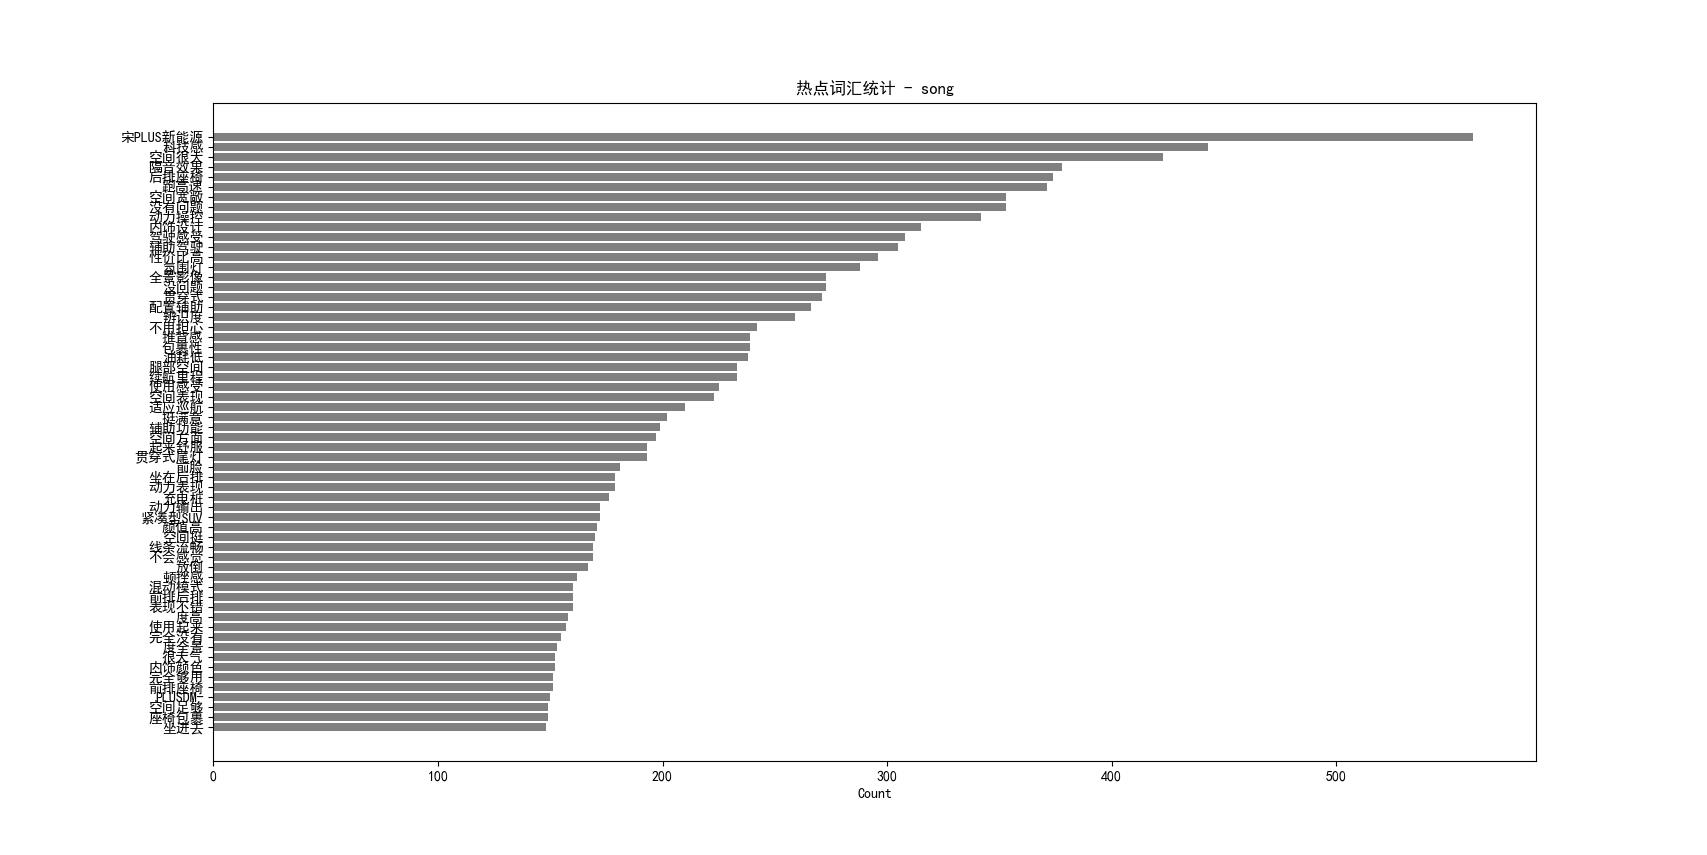
\includegraphics[width=\linewidth]{pictures/54.png}
    \caption{宋PLUS热点词汇统计}
  \end{figure}

  \begin{figure}[htbp]
    \centering
    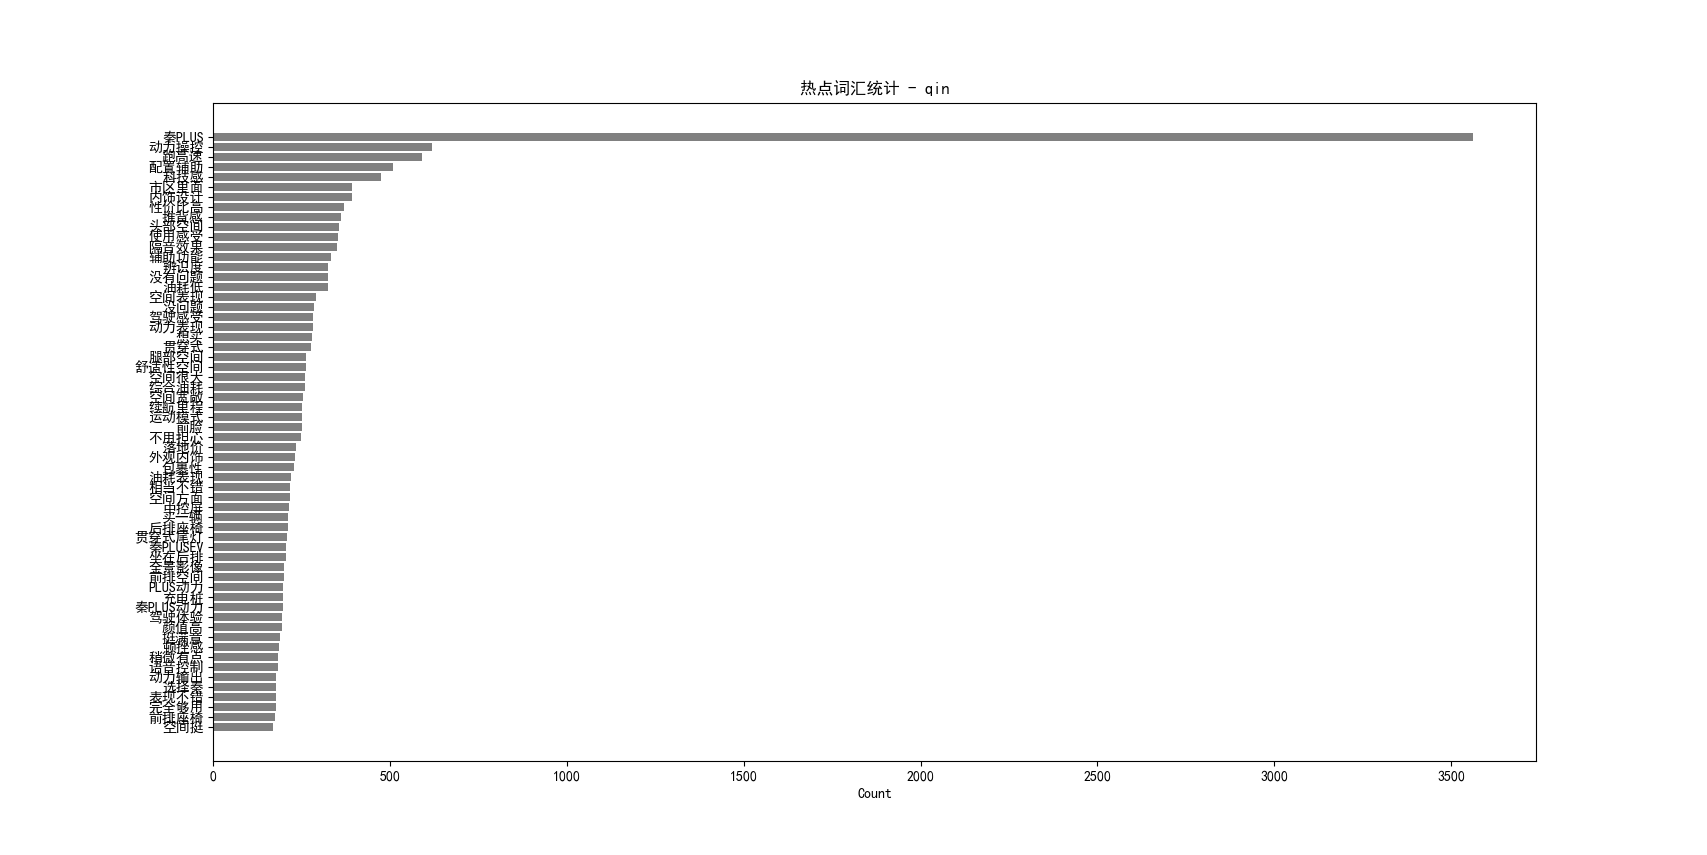
\includegraphics[width=\linewidth]{pictures/55.png}
    \caption{秦PLUS热点词汇统计}
    \end{figure}
  

\subsubsection{总结}

通过上述步骤,我们实现了对汽车评论的热点分析。这一分析不仅帮助我们提取了用户对不同方面的关注点,还通过词云图的方式直观地展示了这些关注点的分布。这对于了解用户需求、改进产品设计以及制定市场策略都具有重要意义。

\subsection{情感分析}

在本实例中,我们采用Text-CNN模型进行情感分析,该模型基于jieba分词和Embedding/Chinese-Word-Vectors知乎回答训练词向量。以下是详细的过程描述:

\subsubsection{数据预处理、分词和词向量}

首先,我们需要对文本数据进行预处理,包括分词和生成词向量。jieba分词是一个常用的中文分词工具,能够将中文文本切分成一个个词语。我们使用jieba分词来处理我们的文本数据。以下是预处理、分词和词向量的具体步骤:

\vskip 0.2cm
\noindent
\textbf{数据预处理:}

1. 读取原始的文本数据,并将其转化为统一的格式。
2. 移除无关字符、空格等噪声数据。

\vskip 0.2cm
\noindent
\textbf{分词:}
1. 使用jieba库对文本数据进行分词,将句子分解成词语序列。
2. 示例代码(python):

\begin{mdframed}[backgroundcolor=darkgray, linecolor=lightgray, linewidth=1pt, innermargin=0.5cm, outermargin=0.5cm, skipbelow=0.1cm]
  \color{white}
  \begin{verbatim}
  def word_cut(text):
  text = regex.sub(' ', text)
  return [word for word in jieba.cut(text) if word.strip()]
\end{verbatim}
  \end{mdframed}

  \vskip 0.2cm
  \noindent
  \textbf{词向量生成:}

1. 我们选择使用预训练的Chinese-Word-Vectors知乎回答训练的词向量,这些词向量是通过大规模知乎数据训练而成,能够捕捉到丰富的上下文信息。

2. 使用词向量将分词后的词语序列转化为向量序列,以便输入到模型中进行训练。

\subsubsection{Text-CNN模型}

由于时间关系,我们选择了纯CNN模型进行情感分析,而没有使用结合BLSTM的CNN模型。结合BLSTM的模型可能效果会更好,但纯CNN模型已经足够满足当前任务的需求。以下是CNN模型的具体原理和参数设置:

\vskip 0.2cm
\noindent
\textbf{模型原理:}

1. Text-CNN模型通过卷积操作提取文本数据中的局部特征。模型中使用了多个不同尺寸的卷积核(filter sizes),以捕捉不同长度的n-gram特征。

2. 卷积层之后是一个最大池化层(Max-Pooling),用于提取重要的特征并降低特征维度。

3. 最后,通过全连接层(Fully Connected Layer)将特征映射到分类标签空间。

\vskip 0.2cm
\noindent
\textbf{模型参数:}

1. 滑动窗口和卷积层:
 
滑动窗口大小(filter sizes):2, 3, 4, 5, 6

卷积核数量(filter num):150

多通道(multichannel):静态和非静态词向量结合使用,以便模型能够根据训练数据微调词向量,从而更好地适应汽车话题。

2. 训练参数:

使用Python命令运行训练脚本,参数设置如下(bash):

\begin{mdframed}[backgroundcolor=darkgray, linecolor=lightgray, linewidth=1pt, innermargin=0.5cm, outermargin=0.5cm, skipbelow=0.1cm]
  \color{white}
  \begin{verbatim}
  python main.py -static=true -non-static=true -multichannel=true -device 0 -pretrained-name ...
\end{verbatim}  
\end{mdframed}


预训练词向量选择知乎bigram,以提高上下文能力。

\vskip 0.2cm
\noindent
\textbf{数据集:}

我们使用了车评相关数据集进行训练从而针对性地提高模型对车评的情感分析能力。数据集含有6300条测试数据及56714条训练数据。示例如下:

\lstinputlisting{car_emotion.txt}

\subsubsection{模型测试}

在训练过程中,我们保存了训练参数(args)、模型参数(best\_model)和词汇表(text\_field\_vocab)。为方便模型的加载和使用,我们封装了一个预测类Predictor,该类负责加载模型、词汇表和训练参数,并提供预测方法。以下是该类的主要功能和实现概述:

\vskip 0.2cm
\noindent
\textbf{加载模型和词汇表}

Predictor 类在初始化时加载训练好的模型参数、词汇表和训练参数,并设置相应的设备(CPU或CUDA)。


\begin{mdframed}[backgroundcolor=darkgray, linecolor=lightgray, linewidth=1pt, innermargin=0.5cm, outermargin=0.5cm, skipbelow=0.1cm]
  \color{white}
  \begin{verbatim}
  class Predictor:
  def __init__(self, model_path='saved/best_model.pt', args_path='saved/args.pkl'...
      print('Loading model...')
      self.device = device
      with open(args_path, 'rb') as f:
          self.args = pickle.load(f)
      if(self.device):
          self.args.device = self.device
      with open(vocab_path, 'rb') as f:
          text_field_vocab = pickle.load(f)
      self.text_field = data.Field(lower=True, tokenize=dataset.word_cut)
      self.text_field.vocab = text_field_vocab
      if self.args.static:
          self.args.embedding_dim = self.text_field.vocab.vectors.size()[-1]
          self.args.vectors = self.text_field.vocab.vectors
      self.model = MD.TextCNN(self.args)
      self.model.load_state_dict(torch.load(model_path))
      if self.args.cuda:
          torch.cuda.set_device(self.args.device)
          self.model = self.model.cuda()
      print('Model loaded')
\end{verbatim}  
\end{mdframed}

该类初始化时:

1. 加载训练参数和词汇表。

2. 根据训练参数和词汇表配置模型。

3. 加载训练好的模型参数,并将模型移动到指定设备上(如CUDA)。

\vskip 0.2cm
\noindent
\textbf{预测方法}

Predictor 类提供 predictstr 方法,该方法接收一系列句子,并返回每个句子的情感预测结果。

\begin{mdframed}[backgroundcolor=darkgray, linecolor=lightgray, linewidth=1pt, innermargin=0.5cm, outermargin=0.5cm, skipbelow=0.1cm]
  \color{white}
  \begin{verbatim}
  class Predictor:
  # ... (上文的初始化代码)

  def predictstr(self, senlist):
      self.model.eval()
      processed_texts = [self.text_field.preprocess(text) for text in senlist]
      tokenized_texts = self.text_field.process(processed_texts).to(self.args.device).t_()
      predictions = []
      with torch.no_grad():
          logits = self.model(tokenized_texts)
          probabilities = F.softmax(logits, dim=-1)
          predicted_labels = torch.max(probabilities, 1)[1]
          predictions.extend(predicted_labels.cpu().numpy())
      return prediction
\end{verbatim}  
\end{mdframed}

该方法具体步骤如下:

1. 预处理

使用 self.Text\_field.preprocess 方法对输入的每个句子进行预处理,包括分词、去除标点等操作。

示例代码:

\begin{mdframed}[backgroundcolor=darkgray, linecolor=lightgray, linewidth=1pt, innermargin=0.5cm, outermargin=0.5cm, skipbelow=0.1cm]
  \color{white}
  \begin{verbatim}
  processed_texts = [self.text_field.preprocess(text) for text in senlist]
\end{verbatim}  
\end{mdframed}

preprocess 将输入文本转化为词语列表,便于后续处理。

2. 词向量化

将预处理后的文本转换为词向量,并转移到指定设备(如GPU)。

示例代码(python):

\begin{mdframed}[backgroundcolor=darkgray, linecolor=lightgray, linewidth=1pt, innermargin=0.5cm, outermargin=0.5cm, skipbelow=0.1cm]
  \color{white}
  \begin{verbatim}
  tokenized_texts = self.text_field.process(processed_texts).to(self.args.device).t_()
\end{verbatim}  
\end{mdframed}

方法将词语列表转换为数值化的词向量序列。

3.	模型预测:

将词向量输入模型,计算输出的logits。

使用Softmax函数将logits转化为概率分布。

通过 torch.max 方法选择最大概率对应的标签作为预测结果。

对应代码(python):

\begin{mdframed}[backgroundcolor=darkgray, linecolor=lightgray, linewidth=1pt, innermargin=0.5cm, outermargin=0.5cm, skipbelow=0.1cm]
  \color{white}
  \begin{verbatim}
    with torch.no_grad():
    logits = self.model(tokenized_texts)
    probabilities = F.softmax(logits, dim=-1)
    predicted_labels = torch.max(probabilities, 1)[1]
\end{verbatim}  
\end{mdframed}

logits 是模型的原始输出值。softmax 将logits转化为概率分布,确保输出的值在0到1之间,且总和为1。torch.max 从概率分布中选取最大值对应的索引,即预测的标签。

4.	结果收集:

将预测结果收集并转换为CPU格式的NumPy数组。

对应代码(python):

\begin{mdframed}[backgroundcolor=darkgray, linecolor=lightgray, linewidth=1pt, innermargin=0.5cm, outermargin=0.5cm, skipbelow=0.1cm]
  \color{white}
  \begin{verbatim}
  predictions.extend(predicted_labels.cpu().numpy())
\end{verbatim}  
\end{mdframed}

  该步骤将GPU上的张量转换为CPU上的NumPy数组,便于后续处理。

  \vskip 0.2cm
  \noindent
  \textbf{情感分析函数}

analyze\_sentiments 函数用于分批次对条评论进行情感分析,并返回带有情感标签的评论列表。该函数利用 Predictor 类中的 predictstr 方法分批处理评论,并在处理过程中显示进度条。

\begin{mdframed}[backgroundcolor=darkgray, linecolor=lightgray, linewidth=1pt, innermargin=0.5cm, outermargin=0.5cm, skipbelow=0.1cm]
  \color{white}
  \begin{verbatim}
  def analyze_sentiments(predictor, comments, batch_size=64):
    sentiments = []
    total_batches = (len(comments) + batch_size - 1) // batch_size
    for i in tqdm(range(total_batches), desc="Analyzing sentiments", unit="batch"):
        batch_comments = comments[i * batch_size:(i + 1) * batch_size]
        sentences = [comment['sentence'] for comment in batch_comments]
        batch_sentiments = predictor.predictstr(sentences)
        sentiments.extend(batch_sentiments)
        for comment, sentiment in zip(batch_comments, batch_sentiments):
            comment['sentiment'] = "正面" if sentiment == 1 else "负面"
    return comments
  \end{verbatim}  
\end{mdframed}

\subsubsection{运行结果}
 
分析成功,得到分类情绪判断,部分实例如下(json):

\begin{mdframed}[backgroundcolor=lightgray!20, linecolor=darkgray, linewidth=1pt]
  \begin{verbatim}
  {
      "sen_id": "296256_1",
      "car_name": "2023款 冠军版 EV 605KM 旗舰PLUS",
      "comment": "方向盘有点轻,感觉开下来没有太好的手感。",
      "aspect": "舒适性",
      "split_id": 3,
      "sentiment": "负面"
  },
  {
      "sen_id": "295971_1",
      "car_name": "2023款 冠军版 EV 520KM 豪华型",
      "comment": "后备箱的空间不大,只能稍微放点小东西,装载能力不太好。",
      "aspect": "空间",
      "split_id": 3,
      "sentiment": "负面"
  },
  {
      "sen_id": "139026_4",
      "car_name": "2021款 DM-i 110KM 旗舰PLUS",
      "comment": "动力很强,尤其是在起步的瞬间。美中不足的就是操控很糟糕",
      "aspect": "操控与性能",
      "split_id": 1,
      "sentiment": "正面"
  },
  {
      "sen_id": "139026_5",
      "car_name": "2021款 DM-i 110KM 旗舰PLUS",
      "comment": "辅助配置非常齐全,360全景也很清晰好用。",
      "aspect": "车机硬件与智能化",
      "split_id": 1,
      "sentiment": "正面"
  },
\end{verbatim}
  \end{mdframed}
    

  \begin{table}[H]
    \centering
    \begin{tabular}{cc}
    \toprule
    情感分类&车评文本\\
    \midrule
    \cellcolor{green!20}正面& "挺时尚风格的一款车子,特别的大气,开出去挺有面子的,...\\
    \cellcolor{red!20}负面& "隔音效果做的并不是很到位,而且这款车子的车机方面稍微有点偏薄了,...\\
    \cellcolor{green!20}正面& "空间方面足够用了,这款车子的前后排空间都是设计非常合理的,...\\
    \cellcolor{green!20}正面& "操控性能挺好的,提速快,平顺性很好。"\\
    \cellcolor{green!20}正面& "是比较有性价比的车子,外观方面非常的给力,...\\
    \cellcolor{red!20}负面& "对于这款车子不满意的,就是速度上来的时候能够听到...\\
    \cellcolor{green!20}正面& "座椅方面还是挺柔软的,而且腰部的支撑性非常的强,...\\
    \cellcolor{green!20}正面& "油耗方面也是比较低的,这款车子它在高速公路上的油耗是不到6个,还是挺划算的。"\\
    \cellcolor{green!20}正面& "感觉这款车子还是挺不错的,尤其是在起步的时候,速度还是比较快的,...\\
    \cellcolor{green!20}正面& "配置方面还是可以的,它的驾驶模式这一块是可以切换的,...\\
    \cellcolor{red!20}负面& "这款车的配置中缺少360度全景影像和中控屏幕尺寸较小。...\\
    \cellcolor{red!20}负面& "馈电状态下启动发动机会有很大的轰鸣声,感觉比较突兀。"\\
    \cellcolor{red!20}负面& "但是车漆有些薄,平常开下来很容易划伤,要特别注意。"\\
    
    \bottomrule
    \end{tabular}
    \caption{车评测试文本的情感分类}
    \end{table}
  
  读入全部车评,得到情感分类统计:


    \begin{figure}[htbp]
    \centering
      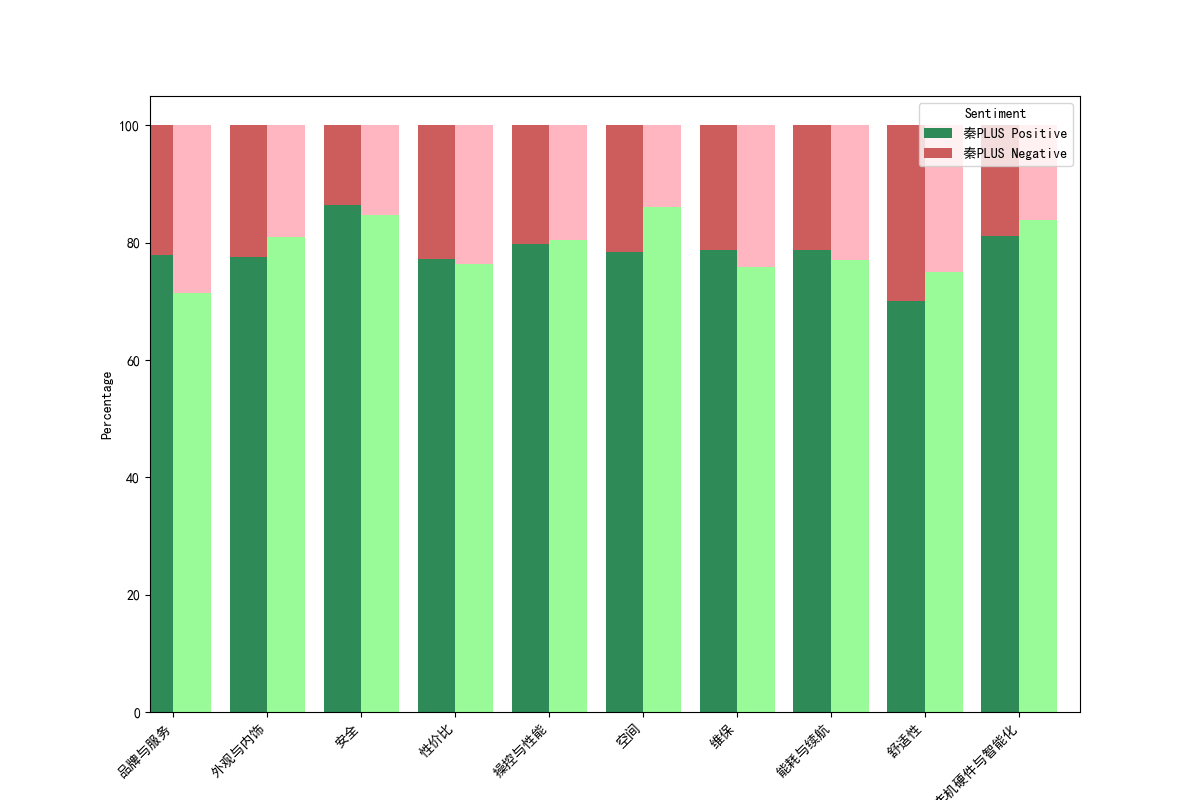
\includegraphics[width=0.8\linewidth]{pictures/53.png}
      \caption{两种车型各类型评论正负面比统计对比}
  
  \end{figure}

\subsubsection{总结}

在情感分析过程中,我们首先对评论文本进行了预处理和分词,并生成了词向量。这些词向量使用了预训练的Chinese-Word-Vectors知乎回答训练模型,以捕捉丰富的上下文信息。接下来,我们训练了一个Text-CNN模型,通过卷积操作提取文本的局部特征,并使用最大池化层和全连接层进行情感分类。训练过程中,我们使用了多通道(multichannel)的词向量设置,以便模型能够根据训练数据微调词向量,从而更好地适应汽车话题。
为了方便模型的加载和使用,我们封装了一个预测类Predictor,该类负责加载训练好的模型参数、词汇表和训练参数,并提供预测方法。通过 Predictor 类,我们能够对输入的评论进行情感预测,并将预测结果添加到评论数据中。整个情感分析过程通过批处理和进度条显示,确保高效和透明。
通过上述步骤,我们实现了对汽车评论的情感分析,为后续的数据展示和综合分析提供了坚实的基础。


\subsection{基于GPT大模型的综合报告}

\noindent
1. 基于时间线的可视化:通过时间线图表展示评论中关键词和情感倾向的变化,直观显示舆情的动态变化。

\noindent
2. 综合分析方法:将提取的热词、评论情感取向及时间线数据喂给GPT等大模型,生成更详细的分析报告,提供更全面的舆情洞察

综合以上程序得到的数据,我们得到两种车型舆情分析报告如下:

\begin{mdframed}[backgroundcolor=morandiLight!30, linecolor=morandiDark, linewidth=1pt]
\begin{center}
  秦Plus和宋Plus车评舆情分析综合报告
\end{center}

\noindent
一、情感分析

通过对比两种车型(秦PLUS 和 宋PLUS 新能源)在不同类别的评论情感,我们可以看到以下结果:

\noindent
\textbf{总体分析}

秦PLUS 的正面情感比例较高,特别是在性价比、空间和动力操控等方面。

宋PLUS 新能源的正面情感比例也较高,但在舒适性和配置与智能化等方面的负面情感比例略高于秦PLUS。

\noindent
\textbf{具体类别分析}

\noindent
性价比:秦PLUS 的正面评论明显高于宋PLUS 新能源,说明消费者对秦PLUS 的价格和性能较为满意。

\noindent
动力操控:两种车型在这一类别上都表现出较高的正面情感,但秦PLUS 的正面比例更高,表明其驾驶体验受到更多消费者的认可。

\noindent
舒适性:宋PLUS 新能源的负面情感比例略高,可能是因为其在舒适性配置或乘坐体验上存在一些不足。

\noindent
配置与智能化:宋PLUS 新能源的负面情感比例较高,可能表明其在智能化配置或车载系统上存在改进空间。

\noindent
二、热点分析

从词云图和热点词汇数量统计柱状图中,可以看出以下趋势:

\noindent
\textbf{秦PLUS}

热点词汇集中在空间、科技感、性价比、动力操控等方面,说明消费者对其在这些方面的表现较为关注和满意。
例如,"跑高速"、"性价比高"、"科技感"等词频率较高,反映出秦PLUS 在这些方面的优势。

\noindent
\textbf{宋PLUS 新能源}

热点词汇集中在空间、科技感、隔音效果、动力操控等方面,说明消费者对其在这些方面也有较高的关注。
例如,"空间宽敞"、"后排座椅空间大"、"科技感"等词频率较高,表明宋PLUS 新能源在这些方面的表现也受到消费者的认可。

\noindent
三、建议

基于以上分析,针对两种车型的营销者提出以下建议:

\noindent
\textbf{秦PLUS 营销建议}

突出性价比:在广告和营销中,强调秦PLUS 在价格和性能方面的优势,吸引预算敏感的消费者。

强化驾驶体验:宣传其在动力操控方面的优异表现,吸引追求驾驶乐趣的消费者。

增强科技感:继续加强其在科技配置上的宣传,如车载系统、智能辅助驾驶等,满足消费者对高科技的需求。

\noindent
\textbf{宋PLUS 新能源营销建议}


改善舒适性:针对舒适性方面的负面反馈,改进座椅设计、隔音效果等,提高整体乘坐体验。

提升智能化配置:加强车载系统和智能化配置的性能,解决消费者在这方面的负面体验,提高用户满意度。

空间利用:在宣传中突出其空间宽敞的优势,吸引注重车内空间的家庭用户。

通过以上针对性的营销策略,可以帮助两种车型的制造商更好地满足消费者需求,提高市场竞争力。

\end{mdframed}

\section{总结与展望}

\subsection{项目创新}

\vskip 0.2cm
\noindent
\textbf{集成分析架构:}论文中提出了一个综合舆情分析系统架构,涵盖数据采集、处理、分析到展示全流程。特别是集成了爬虫技术、分词模型、TF-IDF特征提取、深度学习模型(如BERT和RNN)以及大模型(如GPT)的使用,这种多技术的融合为舆情分析提供了更准确、全面的视角。

\vskip 0.2cm
\noindent
\textbf{深度学习与大模型的应用:}通过应用最新的深度学习技术和预训练的大模型(例如GPT),显著提高了文本数据的情感分析和主题识别的准确性,能够更好地理解复杂的文本内容和上下文关系。

\vskip 0.2cm
\noindent
\textbf{动态趋势预测:}结合时间序列分析模型(如ARIMA),对舆情的发展趋势进行预测,为企业提供决策支持。

\vskip 0.2cm
\noindent
\textbf{交互式数据可视化:}系统通过使用D3.js和Echarts等工具,为用户提供了交互式的图表和报告,使得数据解读更直观、便捷。
  
\subsection{总结}

本研究成功设计并实现了一种智能舆情分析系统,通过综合使用爬虫、自然语言处理、机器学习和大数据技术,有效地从互联网上自动采集和分析数据,识别热点话题和情感倾向,预测舆情趋势。系统的实施不仅提高了数据处理效率,
而且提升了分析的准确性和深度,支持企业在复杂的市场环境中做出更为科学的决策。

\subsection{前景与展望}

\vskip 0.2cm
\noindent
\textbf{模型优化与迭代:}未来研究将继续优化现有的模型,如通过更深层次的学习和调整模型参数,提高模型在特定领域内的准确度和鲁棒性。

\vskip 0.2cm
\noindent
\textbf{数据来源扩展:}扩展数据采集来源,如融合更多类型的社交媒体和网络平台,增加数据的多样性和代表性。

\vskip 0.2cm
\noindent
\textbf{实时数据处理:}改进系统以支持实时数据流的处理,实现舆情动态监控和即时分析。

\vskip 0.2cm
\noindent
\textbf{更多自然语言处理技术的探索:}探索和实验更多先进的NLP技术,如Transformer模型的各种变种,以适应更复杂的语言处理需求。

\vskip 0.2cm
\noindent
\textbf{用户交互与体验改善:}提高系统的用户交互设计,优化报告的生成方式,使非专业用户也能容易理解和操作系统。

通过这些展望,预期能够使舆情分析系统更加精准、高效,更好地服务于企业和公众的需求。

\addcontentsline{toc}{chapter}{参考文献}
\begin{thebibliography}{99}
    \bibitem{ref1} Chen, CF., He, HY., Tong, YX. et al. Analysis of public opinion on employment issues using a combined approach: a case study in China. Sci Rep 14, 1944 (2024). https://doi.org/10.1038/s41598-024-52158-5
    \bibitem{ref2} N. S. Vipin and M. A. Nizar, "A proposal for efficient on-line spam filtering," 2014 First International Conference on Computational Systems and Communications (ICCSC), Trivandrum, India, 2014, pp. 323-327, doi: 10.1109/COMPSC.2014.7032671.
    \bibitem{ref3} Q. Dang Dinh, Q. A. Tran and F. Jiang, "Automated generation of ham rules for Vietnamese spam filtering," the 2014 Seventh IEEE Symposium on Computational Intelligence for Security and Defense Applications (CISDA), Cau Giay, Vietnam, 2014, pp. 1-5, doi: 10.1109/CISDA.2014.7035628.
    \bibitem{ref4} F. Ramadhani, Al-Khowarizmi and I. P. Sari, "Improving the Performance of Naïve Bayes Algorithm by Reducing the Attributes of Dataset Using Gain Ratio and Adaboost," 2021 International Conference on Computer Science and Engineering (IC2SE), Padang, Indonesia, 2021, pp. 1-5, doi: 10.1109/IC2SE52832.2021.9792027.
    \bibitem{ref5} L. Wei, "Genetic Algorithm Optimization of Concrete Frame Structure Based on Improved Random Forest," 2023 International Conference on Electronics and Devices, Computational Science (ICEDCS), Marseille, France, 2023, pp. 249-253, doi: 10.1109/ICEDCS60513.2023.00051.
    \bibitem{ref5} 王佳慧.基于CNN与Bi-LSTM混合模型的中文文本分类方法[J].软件导刊,2023,22(01):158-164.
    \bibitem{ref5} 尹培培.大数据时代的网络舆情分析系统[J].广播与电视技术,2013,40(07):44-47.DOI:10.16171/j.cnki.rtbe.2013.07.029.
    \bibitem{ref5} 李婷.校园BBS舆情分析系统的设计与实现[D].华中科技大学,2009.
    \bibitem{ref5} 杨超,冯时,王大玲,等.基于情感词典扩展技术的网络舆情倾向性分析[J].小型微型计算机系统,2010,31(04):691-695.
    \bibitem{ref5} 党静园.基于深度学习的网络舆情文本倾向性分析系统的研究与设计[D].西安电子科技大学,2019.DOI:10.27389/d.cnki.gxadu.2019.003209.
    \bibitem{ref5} 王展,赵征鹏.基于爬虫的高校网络舆情分析系统设计与实现[J].信息与电脑(理论版),2021,33(03):137-139.
    \bibitem{ref5} 刘堃. 基于机器学习的股市舆情分析及其应用研究[D]. 电子科技大学, 2023. DOI:10.27005/d.cnki.gdzku.2023.001966.
    \bibitem{ref5} 王婷,杨文忠. 文本情感分析方法研究综述 [J]. 计算机工程与应用, 2021, 57 (12): 11-24.
    \bibitem{ref5} R. Murali, "An intelligent web spider for online e-commerce data extraction," 2018 Second International Conference on Green Computing and Internet of Things (ICGCIoT), Bangalore, India, 2018, pp. 332-339, doi: 10.1109/ICGCIoT.2018.8753071. keywords: {Web scrapping;web spiders;online prices;Big data;automated data extraction;CPI data;time series data;inflation forecasting;Python},


  \end{thebibliography}


\end{document}
